% Chapter on Asynchronous Distributed Adaptive Gradient
%
% Developed for my Master Thesis at Maastricht University.
% Based on Eugenio Senes's template at the University of Torino.
%
% By Joeri Hermans (joeri@joerihermans.com)
%
% Released under an MIT license. Share, modify and enjoy, but quote the author!

\chapter{Accumulated Gradient Normalization}
\label{chapter:accumulated_gradient_normalization}

This chapter addresses the first contribution of this thesis, which is \emph{accumulated gradient normalization}, or \textsc{agn} in short. We start by laying out the concept and intuition behind accumulated gradient normalization, and show why \textsc{agn} provides the central variable with more efficient updates. Finally, to show our claims, we provide several experiments where we compare \textsc{agn} with different distributed optimizers such as \textsc{donwpour}~\cite{dean2012large}, \textsc{aeasgd}~\cite{zhang2015deep}, and \textsc{dynsgd}~\cite{jiang2017heterogeneity}.

\section{Concept and intuition}
\label{sec:agn_concept}

The main issue with \textsc{downpour}~\cite{dean2012large} is the requirement of constant communication with the parameter server after every gradient computation. Furthermore, as the number of parallel workers increases, \textsc{downpour} fails to converge due to the amount of \emph{implicit momentum}~\cite{implicitmomentum}, as shown in Figure~\ref{fig:downpour_convergence}. To reduce the amount of communication with the parameter server, one could take ideas from \textsc{easgd}~\cite{zhang2015deep}, and perform several iterations of local exploration before committing the gradients to the parameter server. However, in the case of algorithms like \textsc{downpour}, that is, where gradients are committed to the parameter server in an asynchronous fashion, more local exploration results in proportionally larger gradients, and as a result, complicate the staleness and the implicit momentum problem even further as will be adressed in Chapter~\ref{chapter:asynchronous_distributed_adaptive_gradients}. To intuitively show why this is an issue, let us consider Figure~\ref{fig:downpour_accumulation_issue}. In a regular \textsc{downpour} setting, first-order gradients such as in Subfigure (a) are committed to the parameter server. However, when an algorithm allows for a certain amount of local exploration, such as Algorithm~\ref{algo:downpour_worker_zealous}, the gradient that is committed to the parameter server is an \emph{accumulated gradient} as shown in Subfigure (b).

\begin{figure}[H]
  \centering
  \begin{subfigure}{.49\textwidth}
    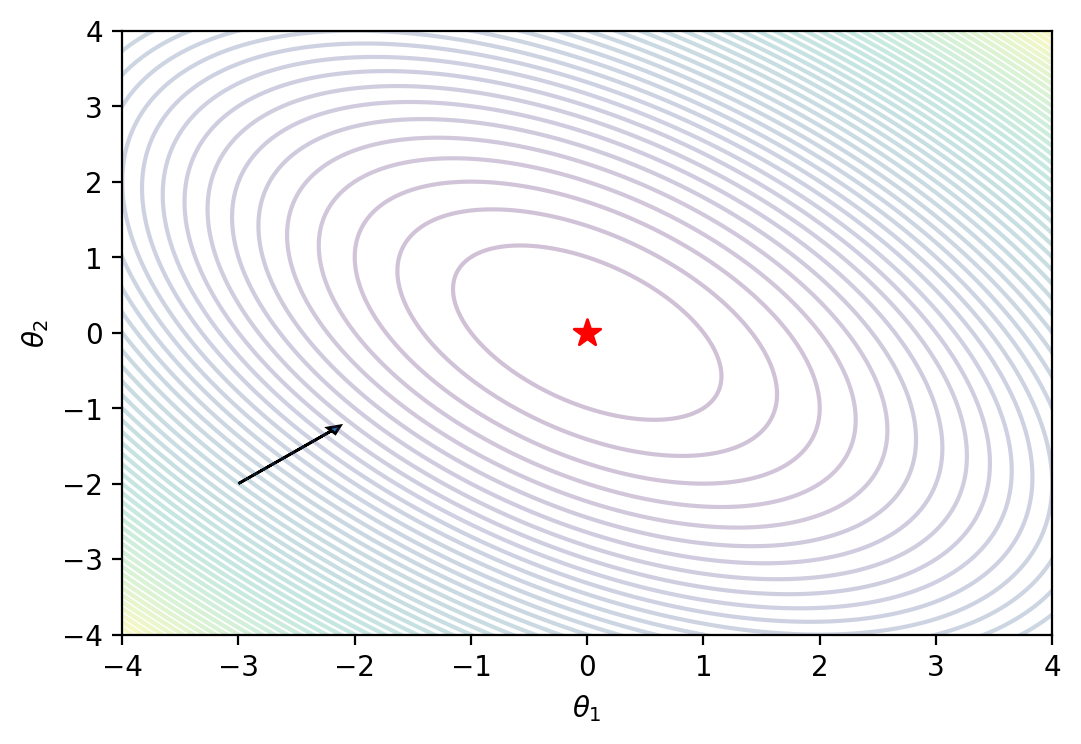
\includegraphics[width=\linewidth]{resources/images/agn_no_accumulated}
    \caption{No Gradient Accumulation}
  \end{subfigure}
    \begin{subfigure}{.49\textwidth}
    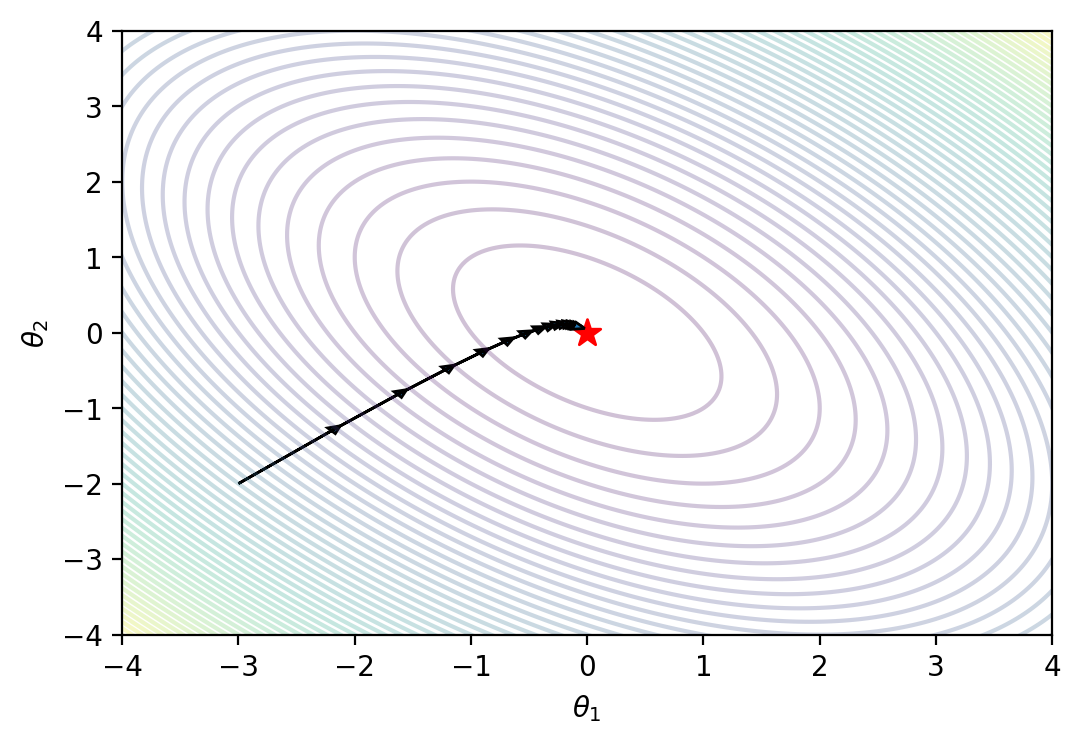
\includegraphics[width=\linewidth]{resources/images/agn_accumulated}
    \caption{Gradient Accumulation}
  \end{subfigure}
  \caption{This figure shows the difference between regular first-order gradients (a), and accumulated gradients (b). We observe that \emph{accumulated gradients are proportionally larger to the number of exploration steps}. However, they do provide a better direction compared to first-order gradients.}
  \label{fig:downpour_accumulation_issue}
\end{figure}

Now, imagine two asynchronous environments, in the first no gradient accumulation is performed, and in the last gradient accumulation takes place. In the environment where no gradient accumulation is performed, as in regular \textsc{downpour}, first-order gradients are committed to the parameter server. However, as we have seen in Chapter~\ref{chapter:distributed_deep_learning}, and in particular Figure~\ref{fig:downpour_convergence}, we saw that \textsc{downpour} diverges when the number of asynchronous workers is too high due to the amount of implicit momentum~\cite{implicitmomentum}. As a result, careful tuning is required when no adaptive methods are applied. Nevertheless, given the fact that \textsc{downpour} converges with $n = 10$ workers in Figure~\ref{fig:downpour_convergence} and our knowledge about gradient accumulation, i.e., \emph{accumulated gradients that are committed are proportional to the number of exploration steps for every worker, and provide better directions to a minimum}, we would expect that for some amount of local exploration while using the same hyperparameterization (with the exception of local exploration steps $\lambda$) \textsc{downpour} would diverge again due to the magnitude of the accumulated gradients. This behaviour is illustrated in Figure~\ref{fig:downpour_accumulated_divergence}.\\

\begin{figure}[H]
  \centering
  \begin{subfigure}{.49\textwidth}
    \centering
    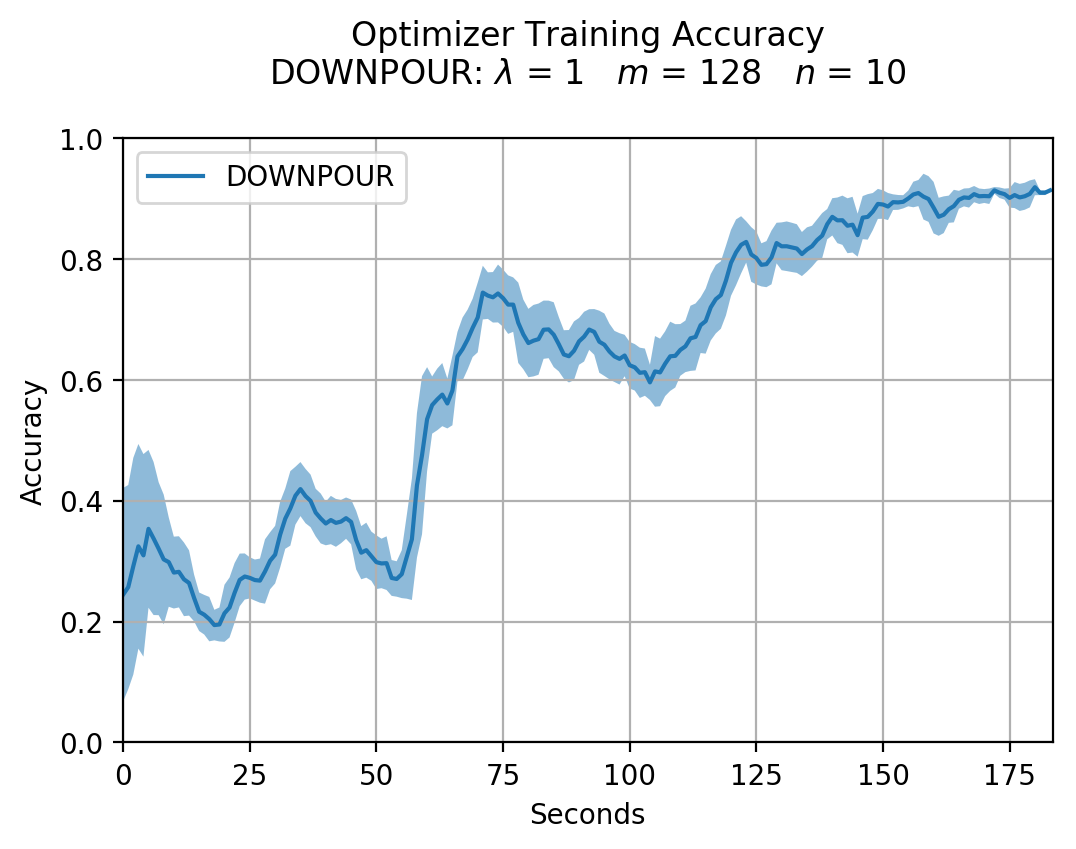
\includegraphics[width=\linewidth]{resources/images/downpour_10}
    \caption{$\lambda = 1$}
  \end{subfigure}
  \begin{subfigure}{.49\textwidth}
    \centering
    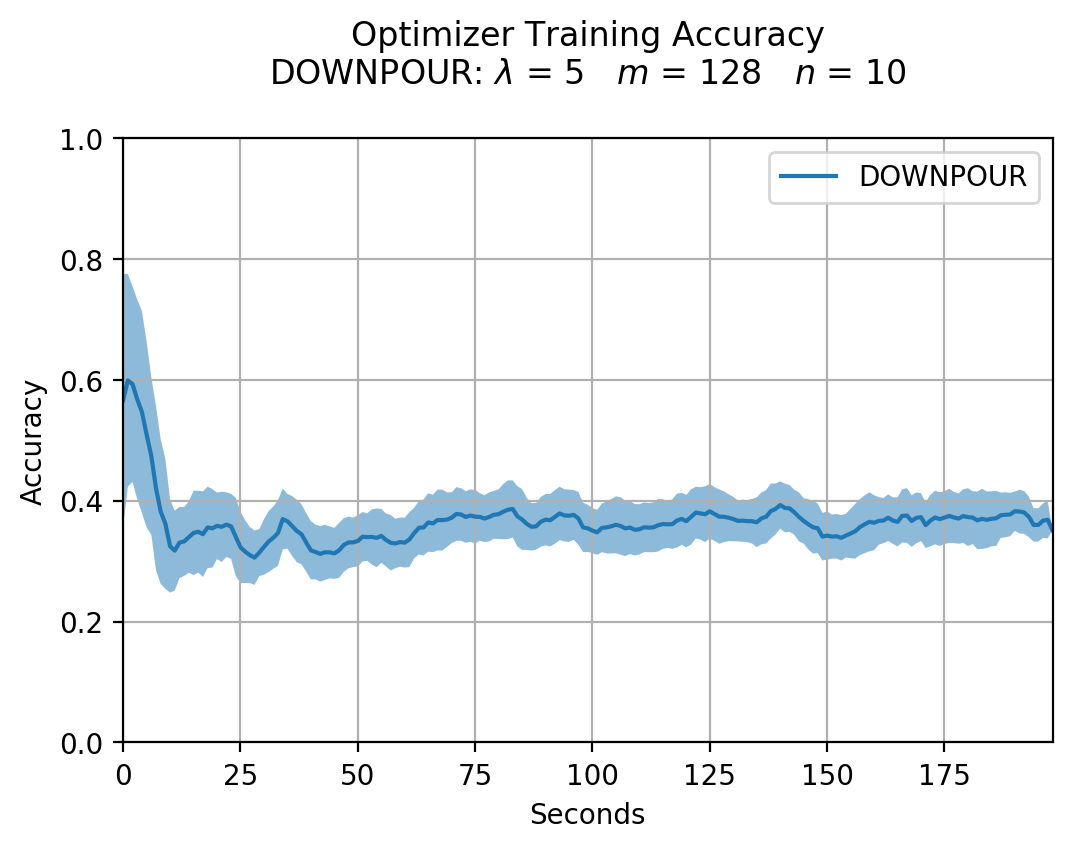
\includegraphics[width=\linewidth]{resources/images/downpour_accumulated_5}
    \caption{$\lambda = 5$}
  \end{subfigure}
   \begin{subfigure}{.49\textwidth}
    \centering
    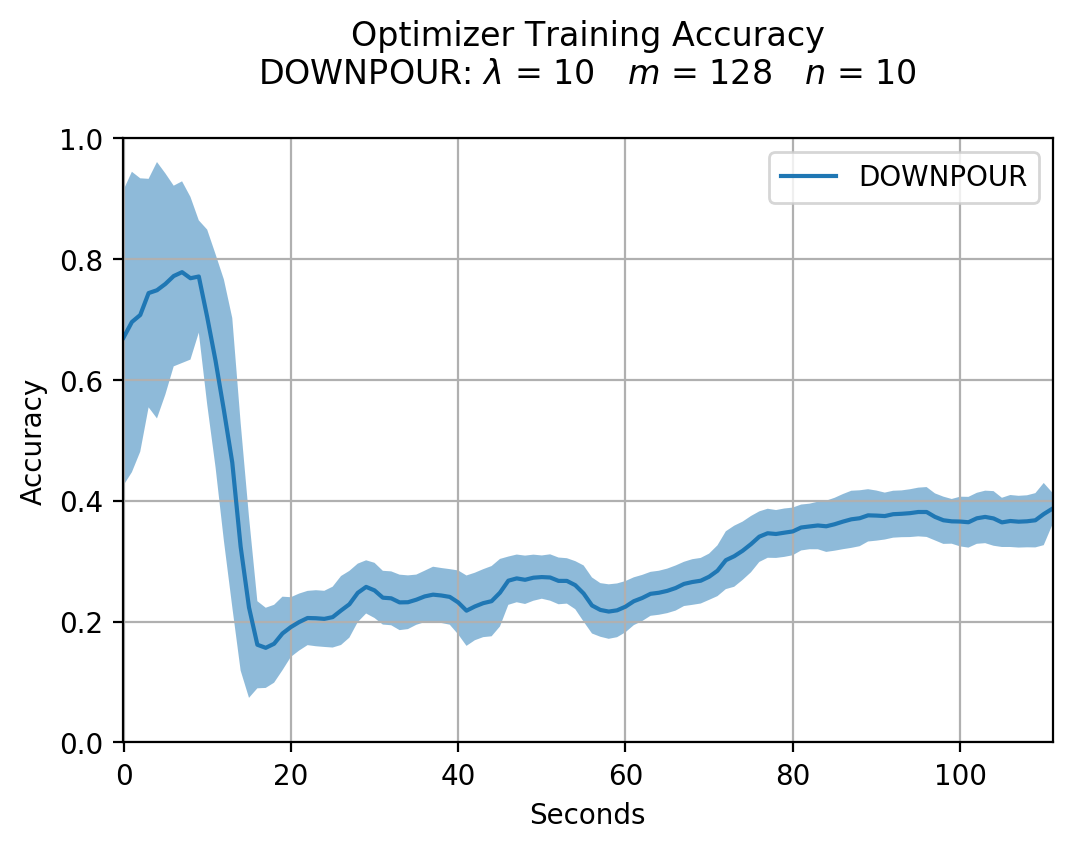
\includegraphics[width=\linewidth]{resources/images/downpour_accumulated_10}
    \caption{$\lambda = 10$}
  \end{subfigure}
  \begin{subfigure}{.49\textwidth}
    \centering
    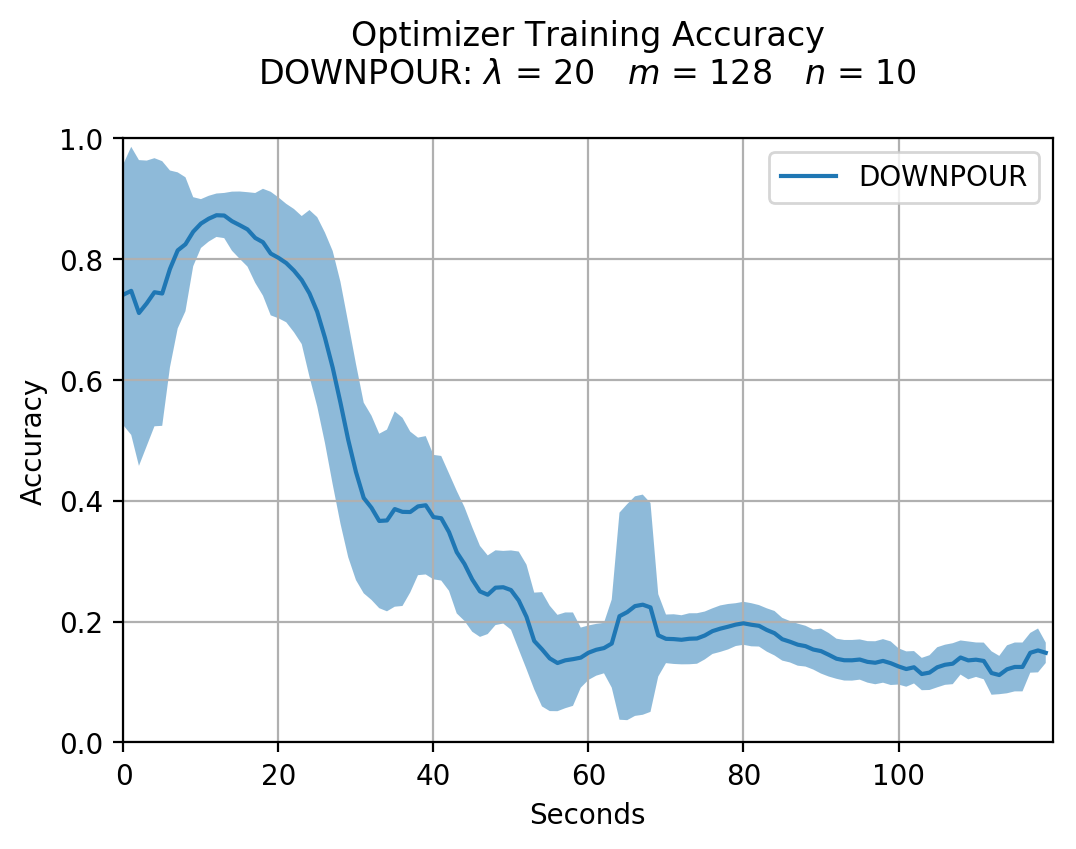
\includegraphics[width=\linewidth]{resources/images/downpour_accumulated_20}
    \caption{$\lambda = 20$}
  \end{subfigure}
  \caption{Illustration of divergence due to gradient accumulation in \textsc{downpour}. In Figure~\ref{fig:downpour_convergence}, we say that for $n = 10$ \textsc{downpour} converged to a good solution. In order to reduce the training time, we decrease the communication frequency (increasing $\lambda$). However, due to the larger gradients that are committed to the parameter server, which increases the amount of implicit momentum, the central variable is not able to converge as before.}
  \label{fig:downpour_accumulated_divergence}
\end{figure}

To reduce the magnitude of the accumulated gradients, and thereby reducing the amount of implicit momentum, while at the same time preserving the better direction that has been provided due to the amount of local exploration, we propose to normalize (average) the accumulated gradient with the amount of local steps that have been performed by the workers ($\lambda$), shown in Equation~\ref{eq:accumulated_gradient_normalization}\footnote{Note if $\lambda = 1$, \textsc{agn} is in essence equivalent to \textsc{downpour}.}. We call this technique of normalizing the accumulated gradient \emph{Accumulated Gradient Normalization} or \textsc{agn}. An initial critique of this technique would be that by normalizing the accumulated gradient, \textsc{agn} would in effect be undoing the work that has been done by a single worker. This seems at first a valid criticism, however, one needs to take into account that \textsc{agn} is actually using the worker exploration steps to compute a better gradient based on first-order gradients.

\begin{equation}
  \label{eq:accumulated_gradient_normalization}
  \Delta\theta = -\frac{1}{\lambda}\sum_{i = 0}^\lambda \eta_t \frac{1}{m}\sum_{j = 0}^{m - 1} \nabla_\theta \mathcal{L}(\theta_i;x_{ij};y_{ij})
\end{equation}

Since \textsc{agn} is using local steps to compute a better gradient compared to first order gradients, it can also be used under communication constraints like \textsc{easgd} since less communication with the parameter server is required. In Figure~\ref{fig:agn_example}, we show how a \emph{Normalized Accumulated Gradient} is obtained and applied to the central variable using Equation~\ref{eq:accumulated_gradient_normalization} as described in Algorithm~\ref{algo:agn}.

\begin{figure}[H]
  \centering
  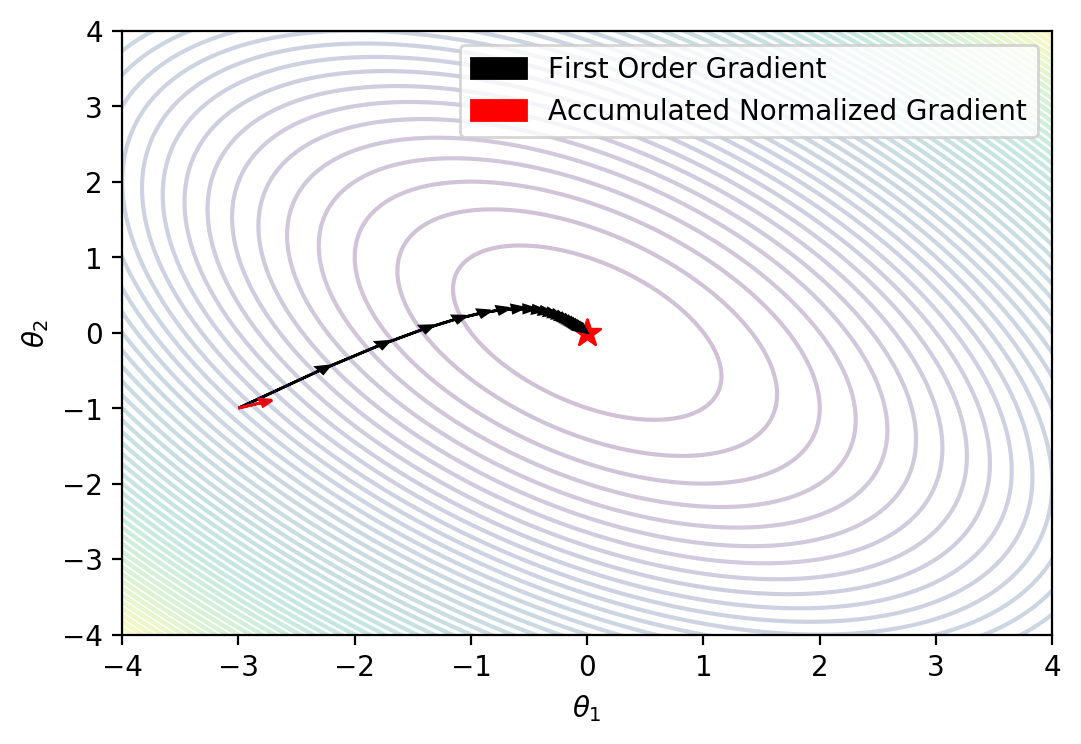
\includegraphics[width=.45\textwidth]{resources/images/agn_example}
  \caption{After pulling the most recent parameterization of the central variable from the parameter server, the worker starts accumulating $\lambda$ first order gradients, and applies those gradients locally to explore the surrounding error space. Finally, after $\lambda$ exploration steps have been performed, the accumulated is normalized w.r.t. $\lambda$ and send to the parameter server.}
  \label{fig:agn_example}
\end{figure}

\begin{algorithm}[H]
  \caption{Worker procedure of \textsc{agn}.}
  \label{algo:agn}
  \begin{algorithmic}[1]
    \Procedure{AGNWorker}{$k$}
    \State $\theta^k_0 \gets \tilde{\theta} \gets \Call{Pull}$
    \State $t \gets 0$
    \While{$\textbf{not}$ converged}
    \State $i \gets 0$
    \State $a \gets 0$
    \While{$i < \lambda$}
    \State $\textbf{x},~\textbf{y} \gets \Call{FetchNextMiniBatch()}{}$
    \State $g \gets -\eta_t \odot \nabla_\theta \mathcal{L}(\theta^k_t;\textbf{x};\textbf{y})$
    \State $a \gets a + g$
    \State $\theta^k_{t + 1} = \theta^k_t + g$
    \State $i \gets i + 1$
    \State $t \gets t + 1$
    \EndWhile
    \State $a \gets \frac{a}{\lambda}$ \Comment{Accumulated Gradient Normalization step.}
    \State $\Call{Commit}{a}$
    \State $\theta^k_{t} \gets \Call{Pull}$
    \EndWhile
    \EndProcedure
  \end{algorithmic}
\end{algorithm}

An interesting thought experiment would be what would happen in the case that the workers would not communicate with the parameter server at all, that is, $\lambda = \infty$. How would the normalized accumulated gradients look like in such a situation, described by Equation~\ref{eq:agn_thought_experiment}?

\begin{equation}
  \label{eq:agn_thought_experiment}
  \lim_{\lambda \to \infty} -\frac{\sum_{i = 0}^\lambda \eta_t \frac{1}{m}\sum_{j = 0}^{m - 1} \nabla_\theta \mathcal{L}(\theta_i;x_{ij};y_{ij})}{\lambda}
\end{equation}

In order to completely understand how the worker deltas would look like after $\lambda = \infty$ steps, one first needs to understand the individual components of Equation~\ref{eq:agn_thought_experiment}. The most inner component, $\eta_t \frac{1}{m}\sum_{j = 0}^{m - 1} \nabla_\theta \mathcal{L}(\theta_i;x_{ij};y_{ij})$, is just the computation of a mini-batch using $m - 1$ samples, where index $i$ denotes the current step in the gradient accumulation. Please note that a mini-batch can differ for different values of $i$ as training samples are randomly retrieved from the dataset. After computing the gradient based on the mini-batch, the local model will be updated as $\theta_{i + 1} = \theta_i - \eta_t\frac{1}{m}\sum_{j = 0}^{m - 1} \nabla_\theta \mathcal{L}(\theta_i;x_{ij};y_{ij})$. This process goes on for $\lambda$ steps, while at the end, the accumulated is normalized with respect to $\lambda$.\\

Let us assume we have a smooth convex error space, or a smooth non-convex error space with at least a single minima. Due to the existance of a minima in both cases, first order gradients will eventually converge to, or in the neighbourhood of said minima. Furthermore, we  make the assumption that the hyperparameterization during the training procedure will not change. For instance, no learning rate decay after $x$ number of steps. Under these assumptions, it is trivial to realize that applying gradient descent for $\infty$ steps will cause the parameterization to converge in a minima. Of course, given that the hyperparameterization, and the data allow for convergence to occur. As a result, the term $\sum_{i = 0}^\lambda \eta_t \frac{1}{m}\sum_{j = 0}^{m - 1} \nabla_\theta \mathcal{L}(\theta_i;x_{ij};y_{ij})$ is finite, even after applying $\infty$ steps of mini-batch updates. To simplify our problem, let us denote $\vec{c}$ as the \emph{finite} result of the top term in Equation~\ref{eq:agn_thought_experiment} for $\lambda = \infty$. Therefore, we can write Equation~\ref{eq:agn_thought_experiment} as Equation~\ref{eq:agn_thought_experiment_2}. Furthermore, since $\vec{c}$ is finite, Equation~\ref{eq:agn_thought_experiment_2} can be treated as an instance of $\frac{1}{\infty}$, which approaches 0. Subsequently, Equation~\ref{eq:agn_thought_experiment_2} is 0 in the limit to infinity.

\begin{equation}
  \label{eq:agn_thought_experiment_2}
  \lim_{\lambda \to \infty} - \frac{\vec{c}}{\lambda} = \vec{0}
\end{equation}

This implies that due to the infinitely low communication frequency, the normalized accumulated gradients will basically be $\vec{0}$. However, what is interesting is that the normalized accumulated gradients directly point towards a minima due to the infinite amount of exploration steps that have been performed. Subsequently, one can view a normalized accumulated gradient when $\lambda = \infty$ as a point, but with a direction. Therefore, if we would allow for infinite steps until convergence, the path the central variable would traverse is a straight line towards the minima, as shown in Figure~\ref{fig:agn_straight_line}.

\begin{figure}[H]
  \centering
  \begin{subfigure}{.49\textwidth}
    \centering
    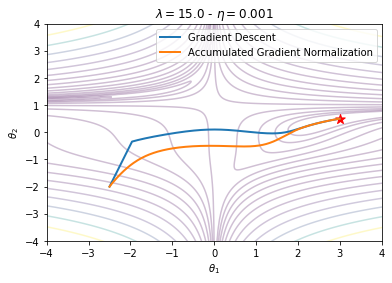
\includegraphics[width=\linewidth]{resources/images/agn_straight_line_1}
    \caption{$\lambda = 15$}
  \end{subfigure}
  \begin{subfigure}{.49\textwidth}
    \centering
    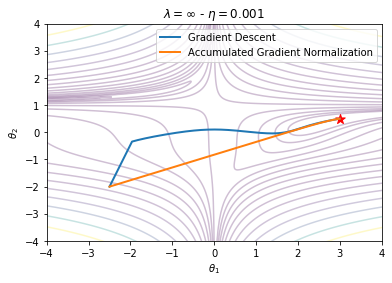
\includegraphics[width=\linewidth]{resources/images/agn_straight_line_2}
    \caption{$\lambda = \infty$}
  \end{subfigure}
  \caption{\textsc{agn} for different values of $\lambda$. This small experiment shows that when $\lambda = \infty$, the path the central variable traverses is equal to a straight line towards the minima.}
  \label{fig:agn_straight_line}
\end{figure}

The thought experiments described above helps us in several ways if make make several additional assumptions. The first assumption assumes that normalized accumulated gradients with $\lambda = \infty$ can be computed immediatly, that is, without a delay. This is of course an unrealistic assumption. However, one needs to consider realistic communication constraints. Given a certain network throughput, what is the amount of local communication that needs to be performed in order for a parameter commit to be ``worth it''. As mentioned above, $\lambda = \infty$ is not a very good solution since the normalized accumulated gradient will converge to $\vec{0}$ in the limit. Nevertheless, if the normalized accumulated gradient could be computed immediately, as we assumed, the central variable would traverse the shortest path to a minima, in contrast to first order gradients. Of course, this is not a realistic assumption. Furthermore, this issue is quite similar to \emph{stochastic gradient descent} vs. \emph{mini-batch gradient descent}, since in \textsc{agn} we also have to make the decision between more frequent parameter updates, and more ``local'' iterations to compute a better gradient, where better in the case of mini-batch gradient descent means less-noisy.\\

In most settings, the size of a mini-batch is determined emperically, and is dependent on the noise of the gradients. Furthermore, when using mini-batch gradient descent, a trade-off is made between more frequent parameter updates, i.e., a smaller mini-batch, or more robust and consistent gradients by increasing the size of a mini-batch which results in a more accurate approximation of the first order curvature. This is similar to our situation. Yet, in mini-batch gradient descent you are basically trying to estimate a hyperparameter based on several unknowns, i.e., convergence based on error space and noise of individual gradients. However, \textsc{agn} is balancing the amount of local computation to produce a better gradient, with the throughput of the network, which is a known variable. For instance, imagine a hypothetical communication infrastructure which is able to apply the commits of the workers directly into the workers with no delay. In this situation, one could apply \textsc{downpour}. However, remember from Figure~\ref{fig:downpour_accumulated_divergence} that \textsc{downpour} does not handle an increased amount of asynchronous parallelism ($n = 20$). As a result, even in an ideal situation \textsc{downpour} will not be able to converge due to the amount of implicit momentum.\\

Nevertheless, the situation in \textsc{agn} is different as will become apparent in Section~\ref{sec:agn_experimental_validation}. Contrary to \textsc{downpour}, \textsc{agn} does not commit first order gradients to the parameter server, but rather a normalized sequence of first order gradients which result in better directions towards a minima, as discussed above. Because of this, workers will produce a better gradient in terms of direction with respect to first order gradients using the amount of local computation available to them to handle the communication constraints. Therefore, \textsc{agn} worker deltas will therefore point more or less in the same direction, and are normalized with respect to the number of exploration steps, which reduces the amount of implicit momentum since first order gradients are not applied to the central variable.

\section{Experimental Validation}
\label{sec:agn_experimental_validation}

In this Section we evaluate \textsc{agn} against different distributed optimization algorithms. As before, MNIST~\cite{mnist} is used as a benchmark dataset, and all optimizers use the model described in Appendix~\ref{appendix:mnist_model} with identical parameterization of the weights. Furthermore, we will set the mini-batch size to $m = 128$ in all optimizers, and use \emph{40 epochs} worth of training data that will be equally distributed over all $n$ workers with the exception for \textsc{downpour}, which will only use 5 epochs, since \textsc{downpour} can not handle accumulated gradients. Our computing infrastructure consists a relatively small cluster of \emph{15 nodes} with a \emph{10Gbps interconnect}, most of them in the same rack, each having 2 Intel\textsuperscript{\textregistered} Xeon\textsuperscript{\textregistered} CPU E5-2650 v2 @ 2.60GHz CPU's, where every CPU has 8 cores and 2 threads. No GPU's are used during training, and no learning rate decay is applied.\\

Our initial experiment, shown in Figure~\ref{fig:agn_experiment_1}, shows the training accuracy of \textsc{agn}, \textsc{aeasgd}, and \textsc{dynsgd} over time. In this experiment, we use a near-optimal hyperparameterization for all optimizers to ensure convergence. Furthermore, we also report the validation accuracy of every trained model based on the validation set that is provided by MNIST. Looking at Figure~\ref{fig:agn_experiment_1}, we observe a significant increase in training performance for \textsc{agn}, both in training accuracy, and in training time when compared to current state-of-the-art algorithms such as \textsc{aeasgd} and \textsc{dynsgd}. Furthermore, the clain we made in Chapter~\ref{chapter:distributed_deep_learning} that \textsc{dynsgd} scales the gradients down with respect to staleness $\tau$, which in effect is $\textbf{E}[\tau] = n - 1$, and thereby not addressing the staleness problem since the expected scaling factor is $(n - 1)^{-1}$ and not the distance between the parameterization of the central variable, and the parameterization of the worker, can be derrived from Figure~\ref{fig:agn_experiment_1} and Figure~\ref{fig:agn_experiment_1} (b). Since gradient accumulation is performed in both figures, i.e., $\lambda > 1$, we can tell that \textsc{dynsgd} has difficulities converging when $\lambda$ is larger because the gradients that are committed to the parameter server are proportionally larger, as is the case in Figure~\ref{fig:agn_experiment_1} (a). Furthermore, due to the relatively high communication frequency ($\lambda = 10$), \textsc{dynsgd} will take longer to process all data since more communication with the parameter server is required. However, in the case of Figure~\ref{fig:agn_experiment_1} (a), we see that \textsc{dynsgd} is equally \emph{temporal efficient} to \textsc{aeasgd}, since \textsc{dynsgd} takes the \emph{same} amount of time to reach the final training accuracy of \textsc{aeasgd}.

\begin{figure}[H]
  \centering
  \begin{subfigure}{.49\textwidth}
    \centering
      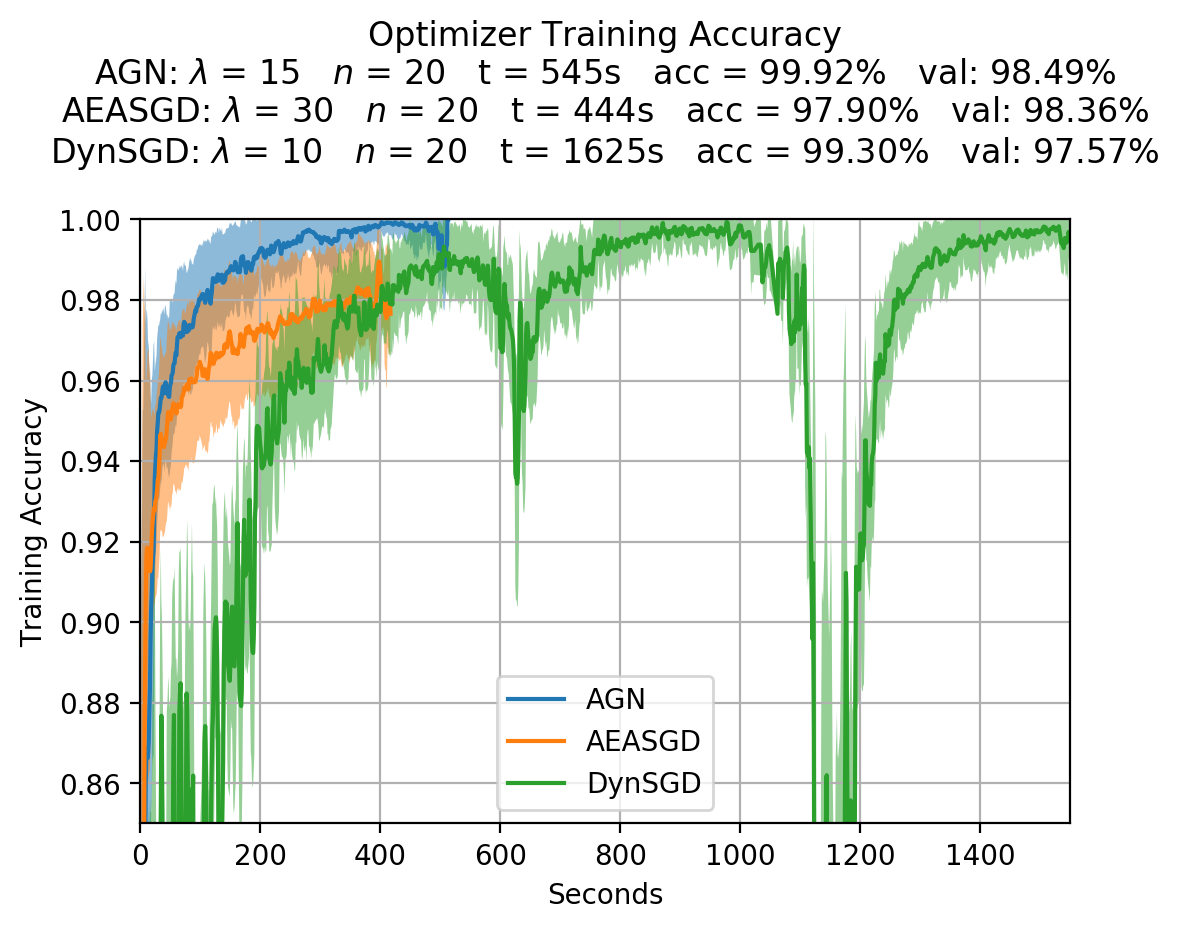
\includegraphics[width=\textwidth]{resources/images/agn_experiment_1}
      \caption{\textsc{dynsgd} $\lambda = 10$}
  \end{subfigure}
  \begin{subfigure}{.49\textwidth}
    \centering
      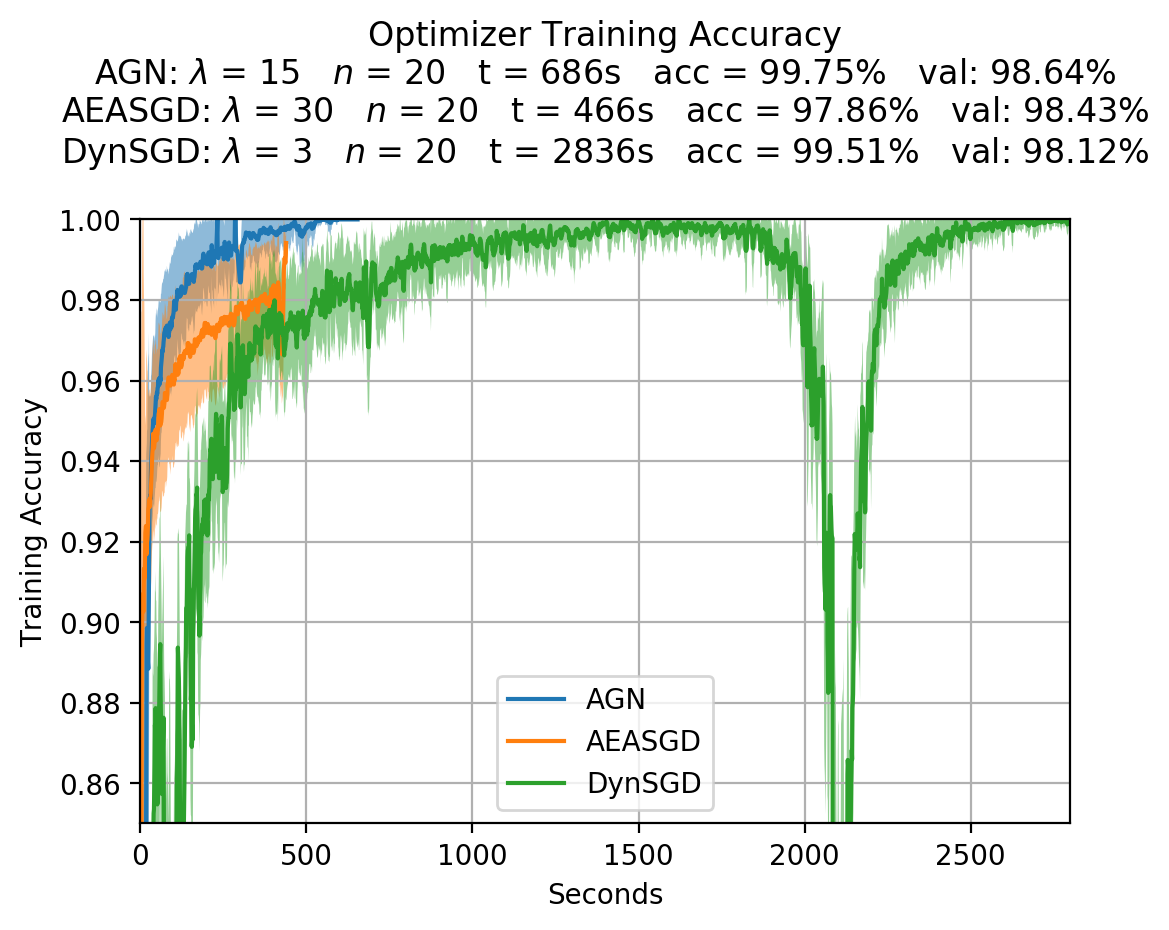
\includegraphics[width=\textwidth]{resources/images/agn_experiment_2}
      \caption{\textsc{dynsgd} $\lambda = 3$}
  \end{subfigure}
  \caption{In this experiment we train all optimizers on 40 epochs worth of data with a mini-batch of $m = 128$. Due to staleness-handling method of \textsc{dynsgd}, the optimizer is not able to handle accumulated gradients which results in non-stale accumulated gradients being incorperated directly into the central variable with the disadvantage that other workers are even more stale in terms of parameter distance. Which is the root cause of this divergent behaviour. In Subfigure (b) we reduce the amount of local exploration steps, which in turn reduces the length of the accumulated gradient. Therefore causing other workers to be less stale, and consequently reducing the divergent effects we observed in Subfigure (a). Furthermore, in Chapter~\ref{chapter:distributed_deep_learning}, we made that claim that \textsc{aeasgd} will not be able to get close to a minima due to the existence of an equilibrium. This behaviour is confirmed as \textsc{aeasgd} is not able to surpass \textsc{agn} in terms of training accuracy. However, as mentioned in Chapter~\ref{chapter:distributed_deep_learning}, the validation accuracy of \textsc{aeasgd} is usually higher than the training accuracy. This results further strengthens our suggestion that due to the presence of the equilibrium condition, \textsc{aeasgd} will not overfit the data since the optimizer will not be able to come ``close'' to a minima.}
  \label{fig:agn_experiment_1}
\end{figure}

Furthermore, let us consider the case for \textsc{dynsgd} when $\lambda = 15$. In this situation, \textsc{dynsgd} closely resembles \textsc{agn} since, as mentioned above, the worker deltas in \textsc{dynsgd} are scaled down with respect to the staleness $\tau$, which results in an expected scaling factor of $(n - 1)^{-1}$. Whereas in \textsc{agn}, the deltas are always scaled (on worker level) with respect to the communication frequency $\lambda$. As a result, the scaling of worker deltas will be \emph{on average} similar to \textsc{agn}. This begs the question, why do we see such divergent, and noisy behaviour in Figure~\ref{fig:agn_experiment_1}, and especially in Figure~\ref{fig:agn_experiment_2}? The reason for the lies in the combined effect how \textsc{dynsgd} deals with staleness, and due to the precense of gradient accumulation. To illustrate this behaviour, consider the case when a \textsc{dynsgd} worker $w$ is committing an \emph{accumulated gradient}, with staleness 0, i.e., $\tau_w = 0$. In this situation, the parameter server will scale down the gradient with respect to $(0 + 1)^{-1}$, which is 1. As a result, the accumulated gradient that worker $w$ sent to the parameter server will not be scaled down. Of course, this is perfectly reasonable, since there the accumulated gradient that worker $w$ sent was not stale. However, what happens when the other $n - 1$ workers have to commit a gradient? Remember from Equation~\ref{eq:dynsgd_ps} that \textsc{dynsgd} scales the gradients down with respect to the number of \emph{stale steps} $\tau_w$. As we will show in Chapter~\ref{chapter:asynchronous_distributed_adaptive_gradients}, this method is rather naive, because what really matters is the \emph{distance} between updates as suggested in Hypothesis~\ref{hyp:local_optimization}. Since the delta worker $w$ committed was not stale, the full accumulated gradient was incorperated into the central variable, causing it to shift with the full magnitude of the delta. Since the length of an accumulated gradient is proportional to the number of local exploration steps, the deltas of other workers will be proportionally more stale in terms of distance, and therefore causing the divergent behaviour shown in Figure~\ref{fig:agn_experiment_1} and Figure~\ref{fig:agn_experiment_2}.

\begin{figure}[H]
  \centering
  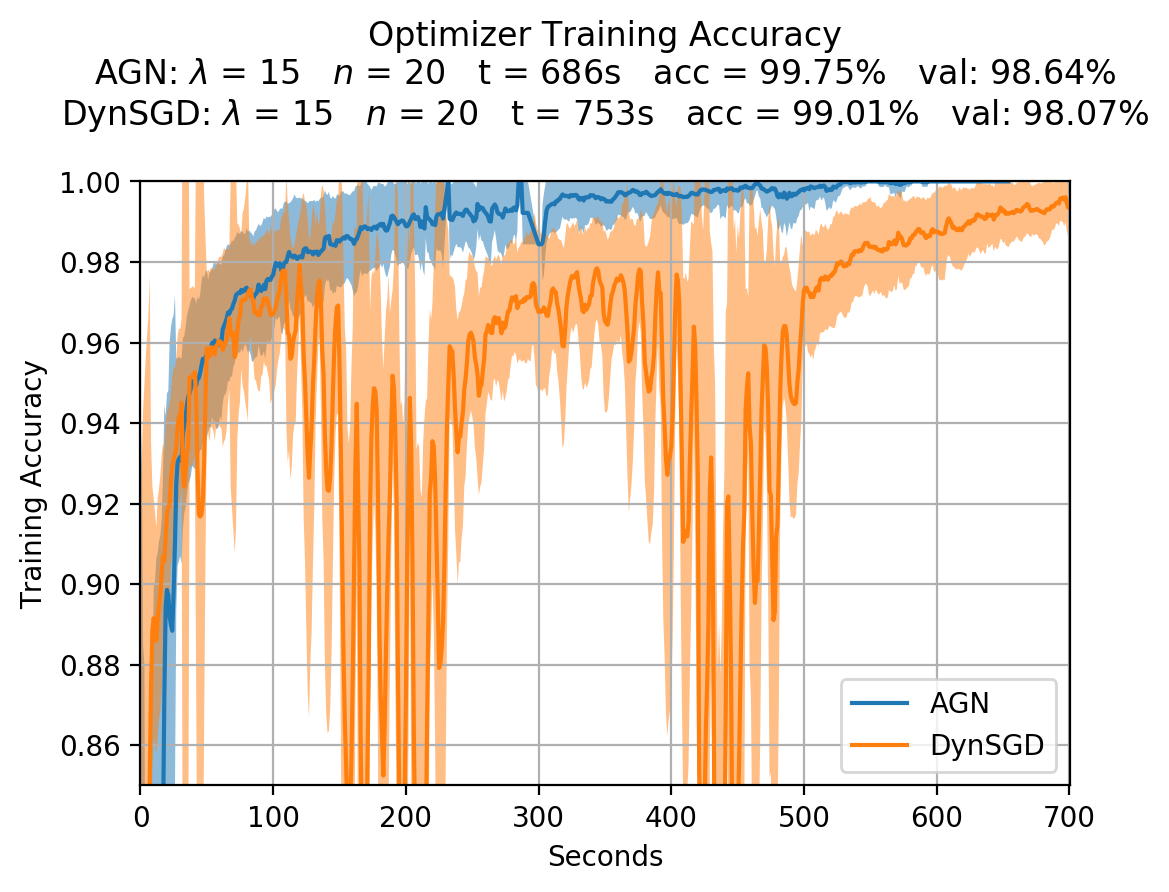
\includegraphics[width=.6\textwidth]{resources/images/agn_experiment_3}
  \caption{Shows the similarity between \textsc{agn} and \textsc{dynsgd} by using identical communication frequencies in both optimizers. As a result, \textsc{dynsgd} worker deltas are \emph{expected} to be similar to \textsc{agn} deltas since $\textbf{E}[\tau] = n - 1$. However, due to \textsc{dynsgd}'s staleness handling mechanism, which is basically scaling the deltas down by the number of \emph{stale steps}, \textsc{dynsgd} is not able to prevent divergent behaviour. Contrary to \textsc{dynsgd}, \textsc{agn} is not staleness aware. However, \textsc{agn} does provide more stable and direct gradient updates since the optimizer normalizes the accumulated gradients proportionally to the amount of local exploration.}
  \label{fig:agn_experiment_2}
\end{figure}

An additional observation from Figure~\ref{fig:agn_experiment_1} and Figure~\ref{fig:agn_experiment_2}, one we made before in Chapter~\ref{chapter:distributed_deep_learning}, is that the validation accuracy of \textsc{aeasgd} is in accordance with the training accuracy, meaning, the optimizer does not seem to overfit. The reason for this lies, according to us, with the \textsc{easgd} equilibrium condition, described in Section~\ref{sec:easgd}. The quilibrium condition will prevent the central variable moving too close to a minima, preventing the central variable from overfitting. Since \textsc{aeasgd} and \textsc{agn} are cleary outperforming \textsc{dynsgd} in terms of training time and validation accuracy for this particular experiment, the following experiments will only consider \textsc{aeasgd} and \textsc{agn}. To evaluate the performance of these optimizers under different conditions, we will conduct several experiments using the same hyperparameterizations we mentioned at the start of this Section, which will evaluate the performance of \textsc{agn} and \textsc{aeasgd} with respect to different (distributed) hyperparameters, i.e., number of workers, and communication frequency. As before, no learning rate decay is applied.\\

Initial observations from our results, summarized in Table~\ref{table:agn_experiments_summary}, indicate that \textsc{agn} performes better in terms of validation accuracy when a low communication frequency is used (which is a design requirement of \textsc{(a)easgd}), and a high number of asynchronous workers are deployed ($n \geq 20$). However, looking at the overall training accuracy of both optimizers, we observe that \textsc{agn} is significantly outperforming \textsc{aeasgd} in all configurations of the distributed hyperparameters. The reason for this might be due to the equilibrium condition of \textsc{easgd} described in Chapter~\ref{chapter:distributed_deep_learning}. Furthermore, increasing the number of asynchronous workers results in a significant drop in both training, and validation accuracy in \textsc{aeasgd}.

\begin{figure}[H]
  \centering
  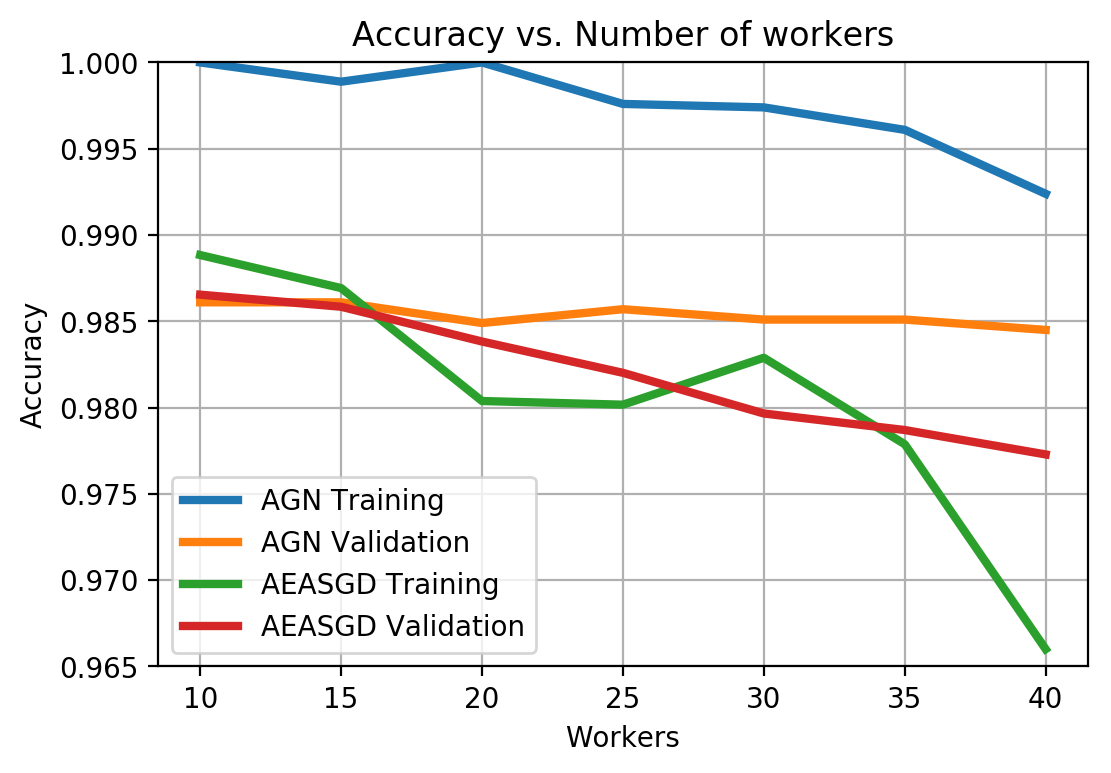
\includegraphics[width=.5\textwidth]{resources/images/agn_aeasgd_workers}
  \caption{Decline of the training accuracy of both \textsc{agn} and \textsc{aeasgd} as the number of asynchronous workers increases. From these experiments, we observe that \textsc{agn} is more rebust to an increased amount of asynchrony as the training accuracy only starts to decrease from $n = 25$ workers, while the validation accuracy remains stable even with 40 workers.}
  \label{fig:agn_aeasgd_workers_performance_decline}
\end{figure}

Contrary to \textsc{aeasgd}, \textsc{agn} is able to cope more effectively with an increased amount of parallelism, as its training accuracy only starts to decline from $n = 25$ asynchronous workers, while the validation accuracy is barely fluctuating (because \textsc{agn} is still slightly overfitting), as shown in Figure~\ref{fig:agn_aeasgd_workers_performance_decline}. An obvious follow-up question to this result would be to question the fact whether increasing the amount of asynchronous workers really improves the temporal efficiency optimizer, i.e., the amount of time it takes to reach a certain training accuracy. In fact, it does reduce the training time to reach a certain training accuracy, as shown in Figure~\ref{fig:agn_temporal_efficiency}. However, several factors have to be taken into account.

\begin{figure}[H]
  \centering
  \begin{subfigure}{.49\textwidth}
    \centering
    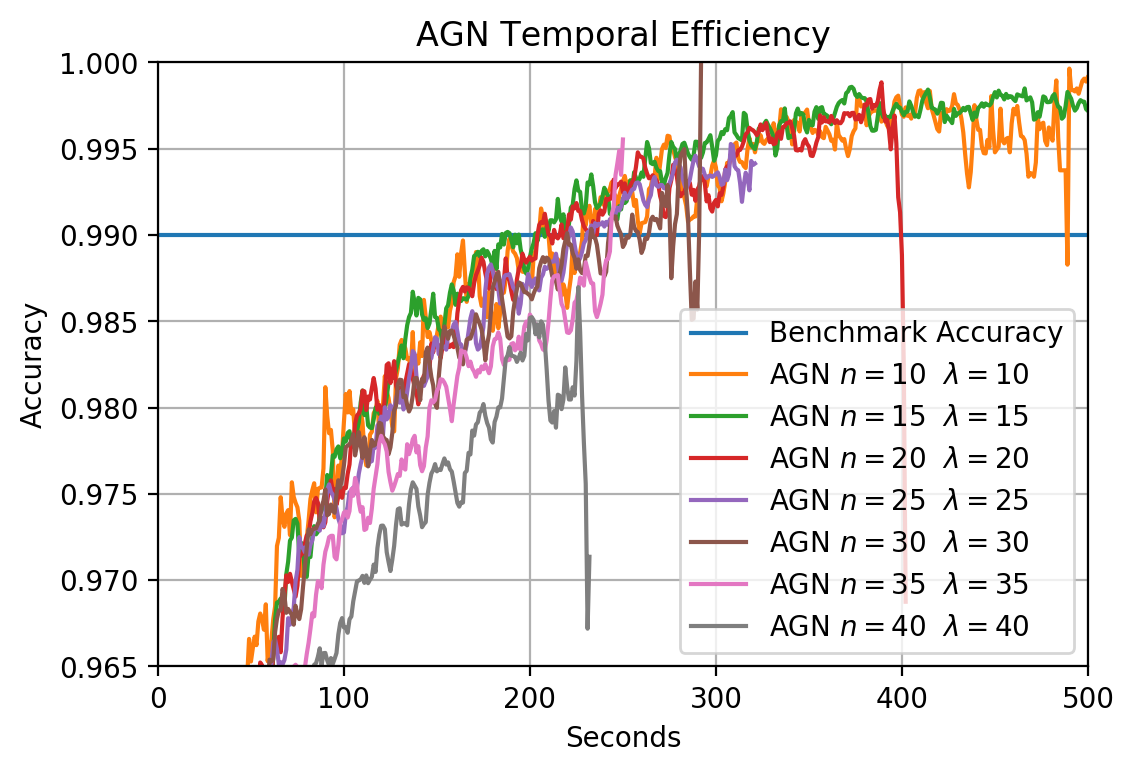
\includegraphics[width=\linewidth]{resources/images/agn_temporal_efficiency}
    \caption{Varying $\lambda$}
  \end{subfigure}
  \begin{subfigure}{.49\textwidth}
    \centering
    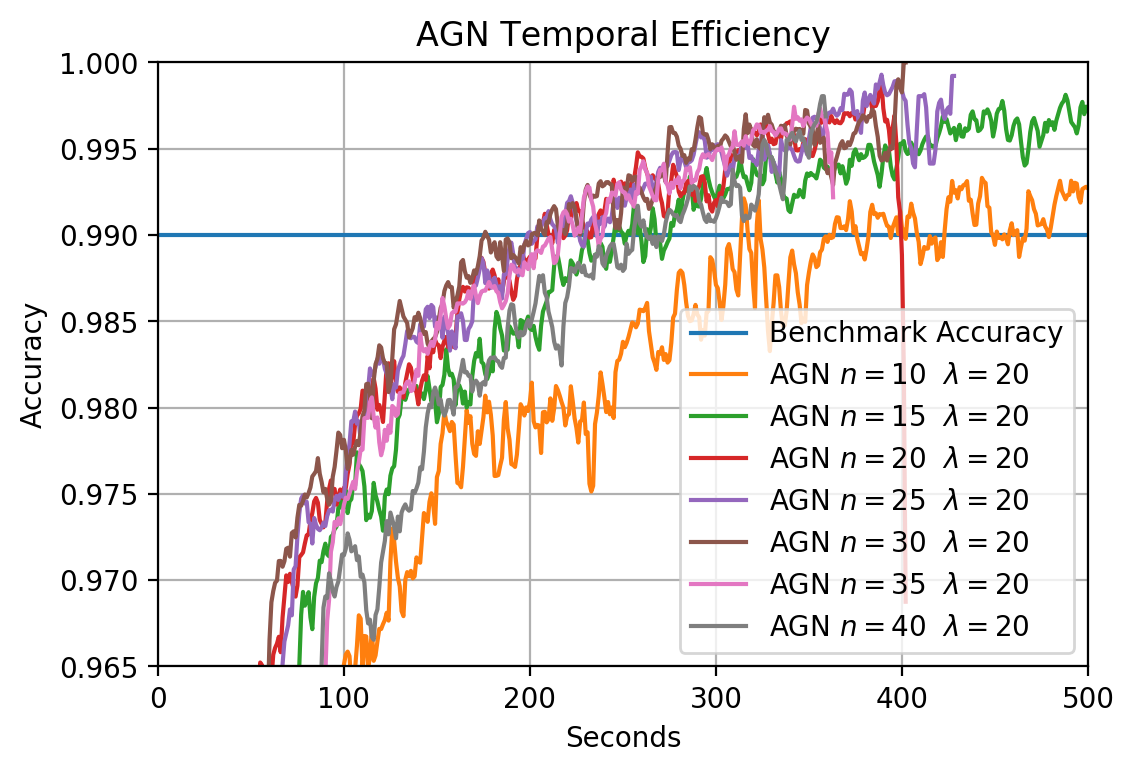
\includegraphics[width=\linewidth]{resources/images/agn_temporal_efficiency_2}
    \caption{Static $\lambda$}
  \end{subfigure}
  \caption{Training accuracy plots for different configurations of the distributed hyperparameters. In the case of a varying $\lambda$ with respect to the number of workers (to minimize the noise of the commits), we observe that optimizers with a higher communication frequency (small $\lambda$), is actually benifitting from the more frequent updates with the parameter server. However, as the number of asynchronous workers grows, a low communication frequency increases the noise in the commits due to parameter staleness. Furthermore, if the $lambda$ is too large, less frequent parameter server updates occur, which results in a slower convergence rate since more time is spent locally. As a result, a balance is required similar to determining the size of a mini-batch.}
  \label{fig:agn_temporal_efficiency}
\end{figure}

The first being an increased amount of staleness that is inserted into the system as the number of asynchronous workers increase. This effect is difficult to mitigate. Previous approaches~\cite{jiang2017heterogeneity} propose to scale gradient commits down proportionally to the number of stale steps. However, as previously shown, this is not an effective solution since accumulating gradients locally, is in effect making the gradients larger, and as a result, committing accummulated gradients increases the \emph{distance} between the central variable and other workers\footnote{Which is our definition of staleness, see Chapter~\ref{chapter:asynchronous_distributed_adaptive_gradients}}. The second and final issue is the balance between updating the central variable with a certain frequency, and the amount of local work to effectively reduce the training time due to high communication costs. In effect, this resembles the situation usually one has when selecting a mini-batch size $m$, i.e., do we allow for more frequent parameter updates (small $m$), or do we compute a less noisy first order gradient by increasing $m$, thereby reducing the frequency of paramter updates and the convergence of a model? To show that this is the case, let us consider Figure~\ref{fig:agn_experiments_workers} and Figure~\ref{fig:agn_experiments_lambdas}. In Figure~\ref{fig:agn_experiments_workers}, we evaluate varying values of $\lambda$ for a specific number of asynchronous workers $n$. In all cases, we observe configurations using $\lambda = 40$ usually have the slowest convergence rate with respect to other configurations with higher communication frequencies. Furthermore, an additional interesting observation, one which is in accordance with the theory we discuss in Chapter~\ref{chapter:asynchronous_distributed_adaptive_gradients}, is the fact that high communication frequencies and a larger number of asynchronous workers causes divergent behaviour due to parameter staleness.\\

Nevertheless, what is really interesting, is why configurations with low communication frequencies actually do converge, in contrast to configurations with high communication frequencies (with respect to the number of workers). Since our definition of staleness relates to the distance between the \emph{current} parameterization of a worker, and the \emph{current} parameterization of the central variable. One can imagine that increasing the number of asynchronous workers, effectively increases the \emph{distance} between the parameterizations of the workers and the \emph{current} central variable due to the queueing model discussed before, i.e., worker deltas are incorperated in the central variable in a queueing fashion. Yet, parameter staleness still does not explain why configurations with low communication frequencies converge, as opposed to configurations with higher communication frequencies. The question begs, is convergence guarenteed due to the amount of local exploration, thus providing the paramater server with a better ``direction'', as shown in Figure~\ref{fig:agn_example}. Or, is it due to limit condition described in Equation~\ref{eq:agn_thought_experiment_2}, which eventually scales the worker deltas down to 0 as the communication frequency decreases ($\lambda$ increases)? This is a rather difficult question to answer. However, we are definitely not dealing with the limit condition since one expects this to be the case when \textsc{agn} approaches a minima, or when $\lambda$ approaches infinity. As a result, the convergence property of \textsc{agn} is largely dedicated to the amount of local exploration, which in turn provides the central variable with a more stable, and direct gradient towards a minima. Alternatively, consider the case when no normalization of the accumulated gradient proportional to the amount of local exploration takes place, and thereby pushing large gradients to the parameter server. We showed that this approached has the tedency to diverge despite the fact it provides a better direction, as is the case in \textsc{agn}. However, due to the magnitude of the worker delta, a lot of staleness (in terms of distance) is induced causing other workers to commit (also large) gradients in an already very stale central variable, which in turn causes the divergence we observe in a non-normalized setting.\\

Now the argument on convergence rates of \textsc{agn} with respect to the communication frequency has been made, let us focus on the influence on the amount of asynchronous workers. For this, we turn to Figure~\ref{fig:agn_experiments_lambdas}, which shows the accuracy plots for several training configurations with a static communication frequency, and a varying number of asynchronous workers. Initial observations indicate that increasing the number of workers with respect to a static communication frequency, speeds up the training procedure. Of course, given the fact that the right communication frequency has been selected in order to ensure convergence. Again, as stated before, lower communication frequencies yield more stable gradients in the precense of more asynchronous workers. However, from Figure~\ref{fig:agn_experiments_workers} and Figure~\ref{fig:agn_experiments_lambdas}, can be deduced that configurations with a lower number of asynchronous workers, and with a high communication frequency actually reach a certain benchmark accuracy faster. Therefore, why spent double the amount of computational resources to achieve the same results?\\

Of course, in such a case one is able to process a lot more training data in a shorter amount of time. However, this is detrimental to the accuracy of the central variable, as more staleness is induced when a larger number of workers is used. Nevertheless, we make this observation for the MNIST~\cite{mnist} dataset. However, if we would use a more challenging dataset such as CIFAR-10(0) or ImageNet, one might actually benefit from an increased amount of parallelism (workers) due to the relatively small parameter updates, which reduces the amount of staleness that workers induce into the central variable.\\

To compare \textsc{agn} against \textsc{aeasgd}, we could take our \emph{temporal efficiency} metric which is described in Chapter~\ref{chapter:introduction}. However, since it basically assumes some \emph{benchmark accuracy} (see Figure~\ref{fig:agn_temporal_efficiency}), the metric might be biased because it requires a person to define a benchmark accuracy. To prevent this issue, we redefine \emph{temporal efficiency} in terms of the surface described by a training metric (be it training accuracy, or training loss). This means that for some optimizer $a$, we have a function $f_a(t)$ which describes the performance of a model at time $t$, e.g., $f_a(t)$ describes the training accuracy of the model at time $t$. If we integrate over $t$, we obtain a surface representing the performance of a model over time. If we would do this for an other optimizer $b$, and divide the surface of optimizer $a$ by the performance surface of optimizer $b$, we get a ratio which describes how optimizer $a$ is performing compared to optimizer $b$. If this ratio is larger then 1, it means that optimizer $a$ is outperforming optimizer $b$, else, it is the other way around (unless the surfaces are equal of course). However, in order to compute a \emph{fair} surface area, we have to limit the computation to the minimum $m$ of both training times. This is done to prevent that optimizers with a longer training time have a significant advantage, since they have more time to produce a better model. To summarize, we define the temporal efficiency $\mathcal{E}$ of two optimizers $a$ and $b$ as the ratio of their peformance surface, as stated in Equation~\ref{eq:temporal_efficiency}. Using this new definition of \emph{temporal efficiency}, we can make a more qualitative judgement which optimizer is performing better in different scenarios.

\begin{equation}
  \label{eq:temporal_efficiency}
  \mathcal{E}(a,b) = \ddfrac{\int_0^m f_a(t) \,dt}{\int_0^m f_b(t) \,dt}
\end{equation}

Finally, we apply the new definition of \emph{temporal efficiency} to compare \textsc{agn} against \textsc{aeasgd} and summarize the results in Table~\ref{table:agn_temporal_efficiency}. However, from Figure~\ref{fig:aeasgd_experiments_workers} and Figure~\ref{fig:aeasgd_experiments_lambdas}, we make the rather strange observation that increasing the amount of asynchrony results in a deterioration of the training accuracy (which is expected since more staleness is induced). However, the rather unexpected property is that increasing the amount of asynchronous workers results in an early \emph{flattening} of the training accuracy. Again, this is due to the equilibrium condition described earlier. Since we increase the amount of asynchrony in the optimization procedure, workers will reach the equilibrium condition faster because the elastic difference is computed based on the most recent parameterization of the central variable. Meaning, as soon as \textsc{aeasgd} is done computing $\lambda$ iterations, the central variable is pulled to the worker where the elastic difference is computed based on the recently pulled central variable, which is very stale (again, using our definition of staleness) due to the low communication frequency and high number of asynchronous workers. As a result, \textsc{aeasgd} has troubles reaching a better training accuracy.

\begin{figure}[H]
  \centering
  \begin{subfigure}{.3\textwidth}
    \centering
    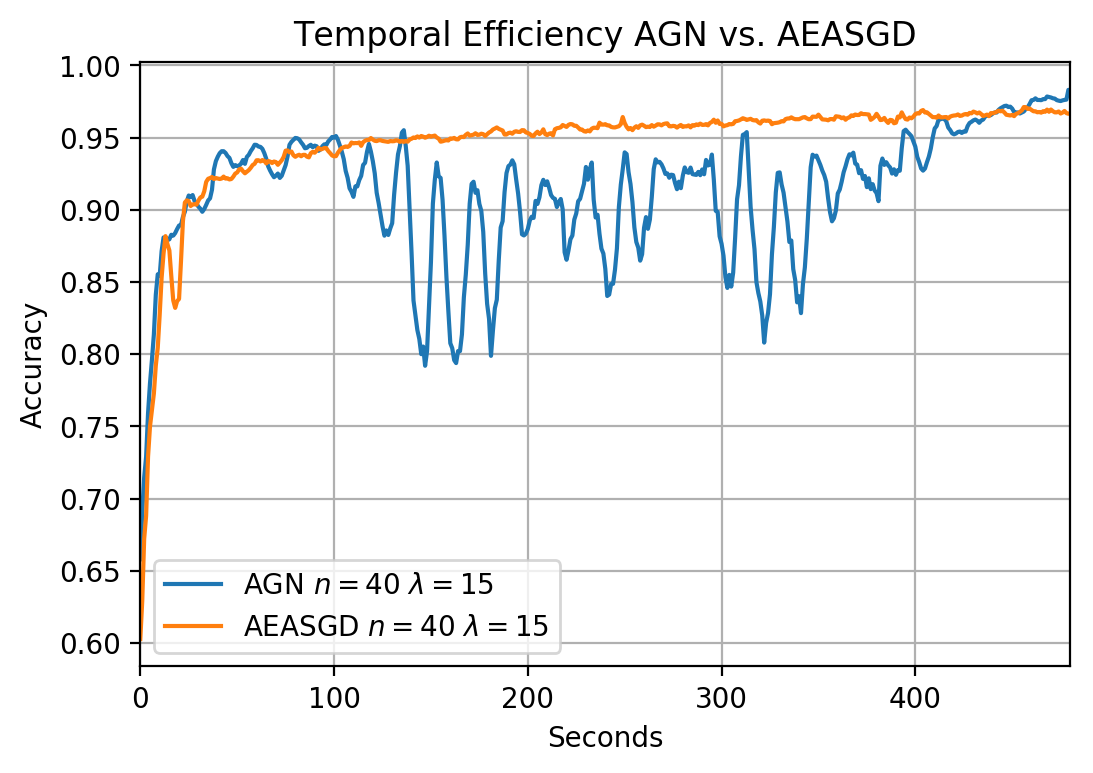
\includegraphics[width=\linewidth]{resources/images/agn_aeasgd_temporal_worst}
    \caption{$\mathcal{E}(\textsc{agn}, \textsc{aeasgd}) = 0.964$}
  \end{subfigure}
  \begin{subfigure}{.3\textwidth}
    \centering
    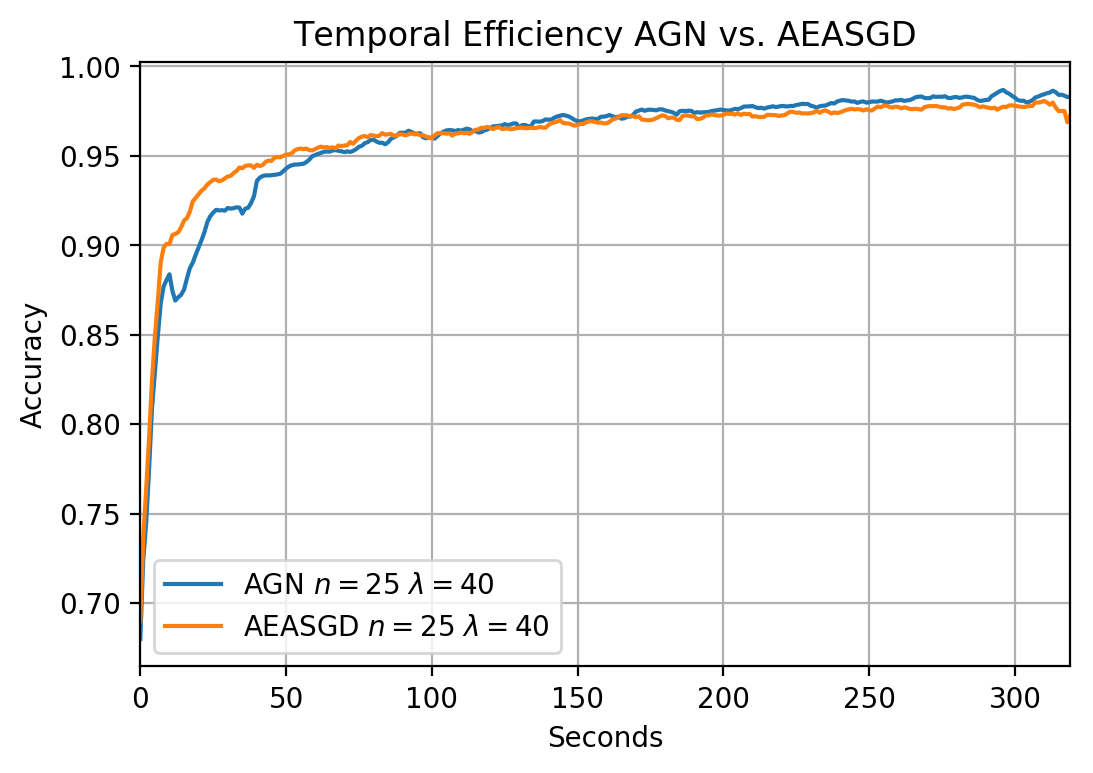
\includegraphics[width=\linewidth]{resources/images/agn_aeasgd_temporal_equal}
    \caption{$\mathcal{E}(\textsc{agn}, \textsc{aeasgd}) = 0.999$}
  \end{subfigure}
  \begin{subfigure}{.3\textwidth}
    \centering
    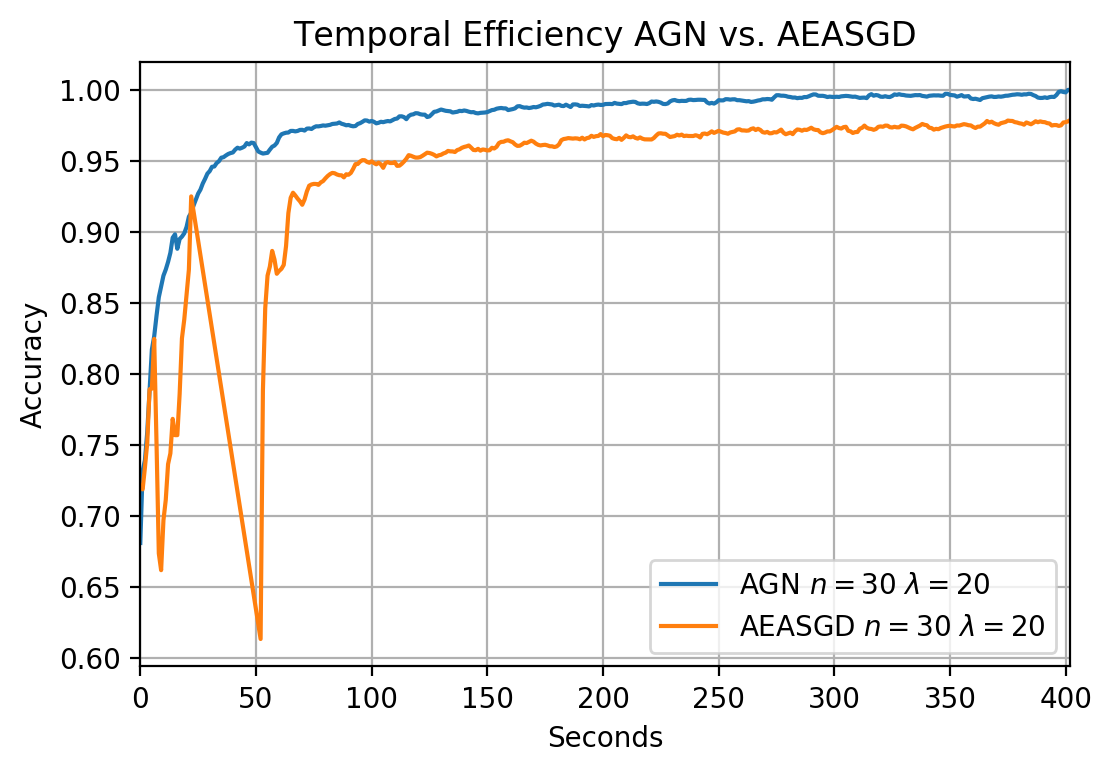
\includegraphics[width=\linewidth]{resources/images/agn_aeasgd_temporal_best}
    \caption{$\mathcal{E}(\textsc{agn}, \textsc{aeasgd}) = 1.044$}
  \end{subfigure}
  \caption{Several accuracy plots of \textsc{agn} and \textsc{aeasgd}. All subfigures show the computed \emph{temporal efficiency} of \textsc{agn}, which were obtained by applying Equation~\ref{eq:temporal_efficiency}.}
\end{figure}

\begin{table}
  \centering
  \begin{tabular}{|c|c|c|}
    \hline
    $n$ & $\lambda$ & Temporal Efficiency \textsc{AGN} \\
    \hline
    \hline
10 & 10 & \textbf{1.009} \\
\hline
10 & 15 & \textbf{1.012} \\
\hline
10 & 20 & \textbf{1.003} \\
\hline
10 & 25 & 0.999 \\
\hline
10 & 30 & 0.988 \\
\hline
10 & 35 & 0.990 \\
\hline
10 & 40 & 0.990 \\
\hline
15 & 10 & \textbf{1.008} \\
\hline
15 & 15 & \textbf{1.015} \\
\hline
15 & 20 & \textbf{1.009} \\
\hline
15 & 25 & \textbf{1.005} \\
\hline
15 & 30 & \textbf{1.000} \\
\hline
15 & 35 & 0.997 \\
\hline
15 & 40 & 0.994 \\
\hline
20 & 10 & 0.983 \\
\hline
20 & 15 & \textbf{1.018} \\
\hline
20 & 20 & \textbf{1.022} \\
\hline
20 & 25 & \textbf{1.009} \\
\hline
20 & 30 & \textbf{1.007} \\
\hline
20 & 35 & \textbf{1.002} \\
\hline
20 & 40 & 0.997 \\
\hline
25 & 10 & 0.954 \\
\hline
25 & 15 & \textbf{1.021} \\
\hline
25 & 20 & \textbf{1.017} \\
\hline
25 & 25 & \textbf{1.014} \\
\hline
25 & 30 & \textbf{1.008} \\
\hline
25 & 35 & \textbf{1.003} \\
\hline
25 & 40 & 0.999 \\
\hline
30 & 10 & 0.926 \\
\hline
30 & 15 & \textbf{1.017} \\
\hline
30 & 20 & \textbf{1.045} \\
\hline
30 & 25 & \textbf{1.015} \\
\hline
30 & 30 & \textbf{1.012} \\
\hline
30 & 35 & \textbf{1.005} \\
\hline
30 & 40 & \textbf{1.005} \\
\hline
35 & 10 & 0.881 \\
\hline
35 & 15 & 0.997 \\
\hline
35 & 20 & \textbf{1.017} \\
\hline
35 & 25 & \textbf{1.020} \\
\hline
35 & 30 & \textbf{1.016} \\
\hline
35 & 35 & \textbf{1.027} \\
\hline
35 & 40 & \textbf{1.012} \\
\hline
40 & 10 & \textbf{1.044} \\
\hline
40 & 15 & 0.964 \\
\hline
40 & 20 & \textbf{1.027} \\
\hline
40 & 25 & \textbf{1.025} \\
\hline
40 & 30 & 0.997 \\
\hline
40 & 35 & \textbf{1.009} \\
\hline
40 & 40 & \textbf{1.009} \\
\hline
  \end{tabular}
  \caption{Temporal efficiency of \textsc{agn} and \textsc{aeasgd} compared to different distributed hyperparameters. Using this information, we can deduce that \textsc{agn} is outperforming \textsc{aeasgd} in 69.73\% of the cases, which is significantly better. Furthermore, this statistic includes cases which are known where \textsc{agn} is performing worse, i.e., small amount of asynchrony, low communication frequency, and high amount of asynchrony, and high communication frequency.}
  \label{table:agn_temporal_efficiency}
\end{table}

\begin{table}
  \centering
  \begin{tabular}{|c|c|c|c|c|c|c|c|}
    \hline
    $n$ & $\lambda$ & \textsc{AGN} $t$ & \textsc{AGN} Acc. & \textsc{AGN} Val. & \textsc{AEASGD} $t$ & \textsc{AEASGD} Acc. & \textsc{AEASGD} Val. \\
    \hline
    \hline
10 & 10 & 1066.08s & \textbf{100.00\%} & 98.43\% & \textbf{953.61s} & 99.22\% & \textbf{98.64\%}  \\
\hline
10 & 15 & 864.01s & \textbf{99.53\%} & 98.54\% & \textbf{846.86s} & 99.38\% & \textbf{98.69\%}  \\
\hline
10 & 20 & 886.34s & \textbf{99.38\%} & 98.61\% & \textbf{804.07s} & 98.91\% & \textbf{98.67\%}  \\
\hline
10 & 25 & 855.51s & 98.75\% & 98.52\% & \textbf{784.46s} & \textbf{98.91\%} & \textbf{98.74\%}  \\
\hline
10 & 30 & \textbf{886.01s} & \textbf{99.22\%} & 98.50\% & 930.73s & 98.91\% & \textbf{98.64\%}  \\
\hline
10 & 35 & 850.87s & 98.44\% & 98.42\% & \textbf{798.74s} & \textbf{99.22\%} & \textbf{98.62\%}  \\
\hline
10 & 40 & 845.21s & \textbf{98.75\%} & 98.43\% & \textbf{791.04s} & 97.66\% & \textbf{98.58\%}  \\
\hline
15 & 10 & 979.72s & \textbf{99.67\%} & 98.61\% & \textbf{813.32s} & 99.11\% & \textbf{98.67\%}  \\
\hline
15 & 15 & \textbf{638.13s} & \textbf{99.89\%} & 98.58\% & 721.47s & 98.66\% & \textbf{98.65\%}  \\
\hline
15 & 20 & \textbf{562.72s} & \textbf{99.89\%} & 98.49\% & 564.92s & 99.00\% & \textbf{98.60\%}  \\
\hline
15 & 25 & 580.71s & \textbf{98.77\%} & 98.50\% & \textbf{542.28s} & 98.33\% & \textbf{98.62\%}  \\
\hline
15 & 30 & \textbf{544.97s} & 98.44\% & 98.44\% & 660.58s & \textbf{98.55\%} & \textbf{98.58\%}  \\
\hline
15 & 35 & \textbf{562.93s} & \textbf{98.66\%} & 98.45\% & 573.54s & 98.33\% & 98.45\%  \\
\hline
15 & 40 & \textbf{561.17s} & \textbf{99.22\%} & 98.42\% & 566.00s & 98.88\% & \textbf{98.52\%}  \\
\hline
20 & 10 & 839.94s & \textbf{99.26\%} & 98.36\% & \textbf{821.12s} & 97.90\% & \textbf{98.52\%}  \\
\hline
20 & 15 & \textbf{571.17s} & \textbf{100.00\%} & 98.45\% & 610.88s & 98.52\% & \textbf{98.49\%}  \\
\hline
20 & 20 & \textbf{432.93s} & \textbf{99.38\%} & \textbf{98.47\%} & 510.72s & 97.78\% & 98.39\%  \\
\hline
20 & 25 & 479.72s & \textbf{99.63\%} & \textbf{98.45\%} & \textbf{421.50s} & 97.86\% & 98.34\%  \\
\hline
20 & 30 & 433.36s & \textbf{99.42\%} & \textbf{98.49\%} & \textbf{429.16s} & 98.36\% & 98.33\%  \\
\hline
20 & 35 & 418.83s & \textbf{98.52\%} & \textbf{98.44\%} & \textbf{409.86s} & 98.19\% & 98.33\%  \\
\hline
20 & 40 & 434.86s & \textbf{98.44\%} & \textbf{98.34\%} & \textbf{420.46s} & 97.66\% & 98.28\%  \\
\hline
25 & 10 & 768.45s & \textbf{98.62\%} & 97.87\% & \textbf{753.27s} & 98.26\% & \textbf{98.40\%}  \\
\hline
25 & 15 & \textbf{524.85s} & \textbf{99.76\%} & \textbf{98.57\%} & 540.20s & 98.32\% & 98.32\%  \\
\hline
25 & 20 & 455.92s & \textbf{99.70\%} & \textbf{98.52\%} & \textbf{401.17s} & 97.66\% & 98.23\%  \\
\hline
25 & 25 & \textbf{351.30s} & \textbf{99.10\%} & \textbf{98.44\%} & 372.74s & 98.44\% & 98.26\%  \\
\hline
25 & 30 & 365.58s & \textbf{98.56\%} & \textbf{98.48\%} & \textbf{364.29s} & 98.20\% & 98.14\%  \\
\hline
25 & 35 & \textbf{364.04s} & \textbf{98.32\%} & \textbf{98.46\%} & 371.01s & 97.54\% & 98.02\%  \\
\hline
25 & 40 & 373.22s & \textbf{98.05\%} & \textbf{98.35\%} & \textbf{346.99s} & 97.72\% & 98.04\%  \\
\hline
30 & 10 & 778.42s & 97.92\% & 97.25\% & \textbf{764.59s} & \textbf{99.17\%} & \textbf{98.28\%}  \\
\hline
30 & 15 & \textbf{507.43s} & \textbf{99.72\%} & \textbf{98.51\%} & 527.42s & 98.12\% & 98.13\%  \\
\hline
30 & 20 & \textbf{428.09s} & \textbf{99.74\%} & \textbf{98.48\%} & 461.58s & 97.92\% & 98.03\%  \\
\hline
30 & 25 & 341.44s & \textbf{99.01\%} & \textbf{98.48\%} & \textbf{334.52s} & 98.59\% & 97.96\%  \\
\hline
30 & 30 & 318.41s & \textbf{99.17\%} & \textbf{98.39\%} & \textbf{310.19s} & 97.66\% & 97.77\%  \\
\hline
30 & 35 & 312.96s & \textbf{99.17\%} & \textbf{98.35\%} & \textbf{305.48s} & 98.28\% & 97.86\%  \\
\hline
30 & 40 & \textbf{316.68s} & \textbf{98.65\%} & \textbf{98.30\%} & 343.07s & 98.28\% & 97.73\%  \\
\hline
35 & 10 & \textbf{691.38s} & 96.65\% & 96.74\% & 785.00s & \textbf{98.09\%} & \textbf{97.96\%}  \\
\hline
35 & 15 & \textbf{511.17s} & \textbf{99.01\%} & \textbf{98.18\%} & 515.88s & 97.91\% & 98.06\%  \\
\hline
35 & 20 & \textbf{390.05s} & \textbf{99.61\%} & \textbf{98.51\%} & 405.90s & 97.77\% & 98.01\%  \\
\hline
35 & 25 & \textbf{314.71s} & \textbf{99.52\%} & \textbf{98.37\%} & 324.66s & 97.82\% & 97.81\%  \\
\hline
35 & 30 & \textbf{273.62s} & \textbf{98.67\%} & \textbf{98.43\%} & 379.93s & 97.63\% & 97.82\%  \\
\hline
35 & 35 & \textbf{276.11s} & \textbf{99.29\%} & \textbf{98.13\%} & 357.71s & 97.50\% & 97.84\%  \\
\hline
35 & 40 & \textbf{284.50s} & \textbf{98.69\%} & \textbf{98.17\%} & 543.86s & 97.79\% & 97.59\%  \\
\hline
40 & 10 & \textbf{748.94s} & 94.17\% & 95.55\% & 1256.09s & \textbf{96.57\%} & \textbf{97.99\%}  \\
\hline
40 & 15 & \textbf{506.25s} & 95.99\% & 97.25\% & 534.42s & \textbf{96.88\%} & \textbf{97.89\%}  \\
\hline
40 & 20 & \textbf{383.51s} & \textbf{99.24\%} & \textbf{98.40\%} & 412.37s & 96.65\% & 97.83\%  \\
\hline
40 & 25 & \textbf{308.15s} & \textbf{98.86\%} & \textbf{98.39\%} & 347.50s & 96.65\% & 97.67\%  \\
\hline
40 & 30 & 351.54s & \textbf{98.66\%} & \textbf{98.45\%} & \textbf{305.50s} & 96.47\% & 97.67\%  \\
\hline
40 & 35 & 279.30s & \textbf{98.73\%} & \textbf{98.32\%} & \textbf{252.70s} & 96.32\% & 97.60\%  \\
\hline
40 & 40 & 257.62s & \textbf{97.88\%} & \textbf{98.18\%} & \textbf{250.74s} & 96.65\% & 97.45\%  \\
\hline
  \end{tabular}
  \caption{Summary of \textsc{agn} and \textsc{aeasgd} experiments using different distributed hyperparameters ($n$ and $\lambda$). From these experiments we find that \textsc{agn} performs better in terms of training, and validation accuracy in the precense of a higher number of asynchronous workers, and a reduced communication frequency.}
  \label{table:agn_experiments_summary}
\end{table}

\begin{figure}
  \centering
  \begin{subfigure}{.3\textwidth}
    \centering
    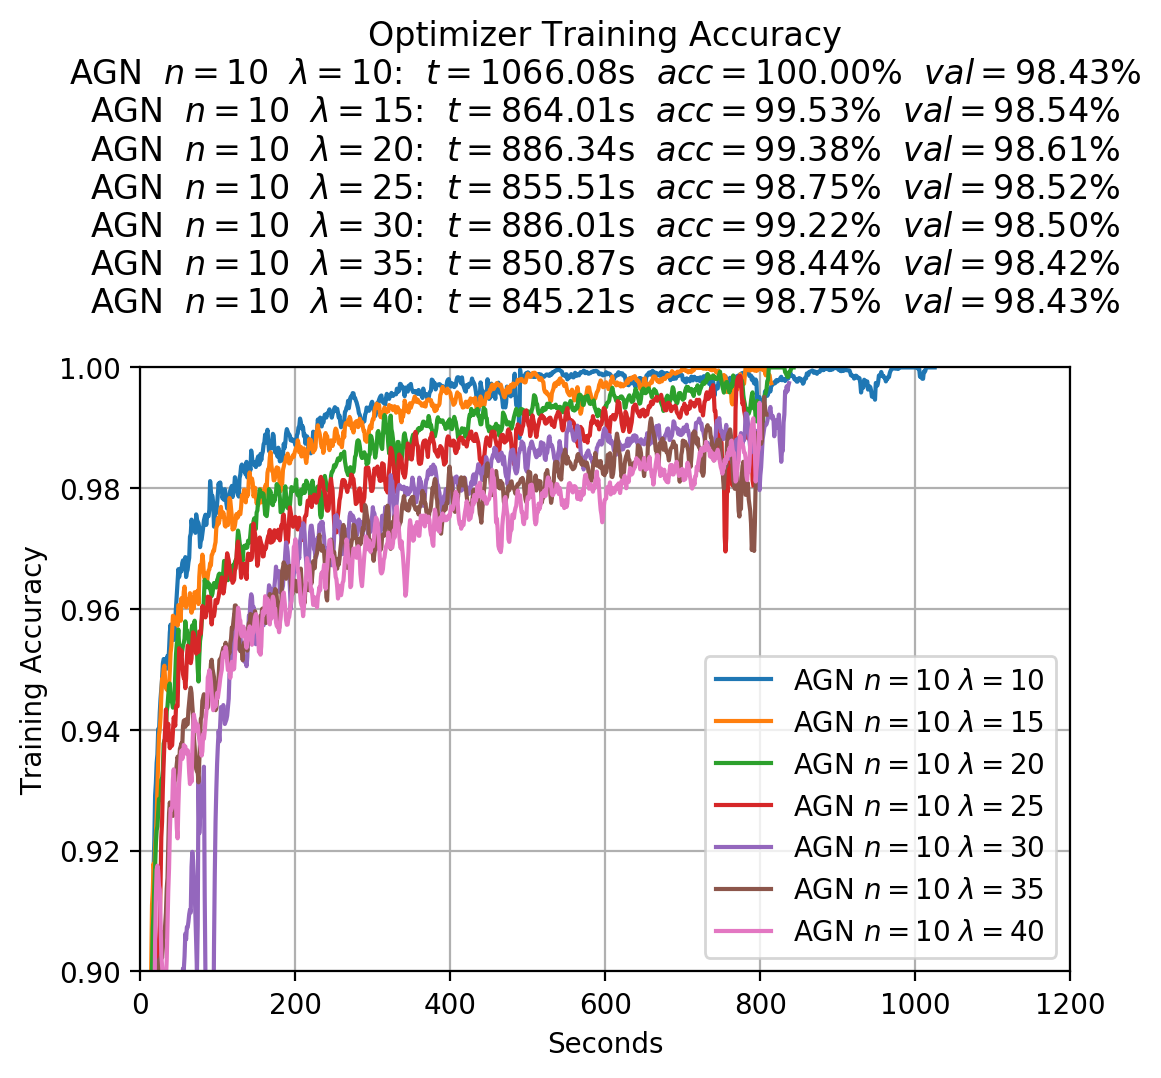
\includegraphics[width=\linewidth]{resources/images/agn_experiments_workers_10}
    \caption{$n = 10$}
  \end{subfigure}
  \begin{subfigure}{.3\textwidth}
    \centering
    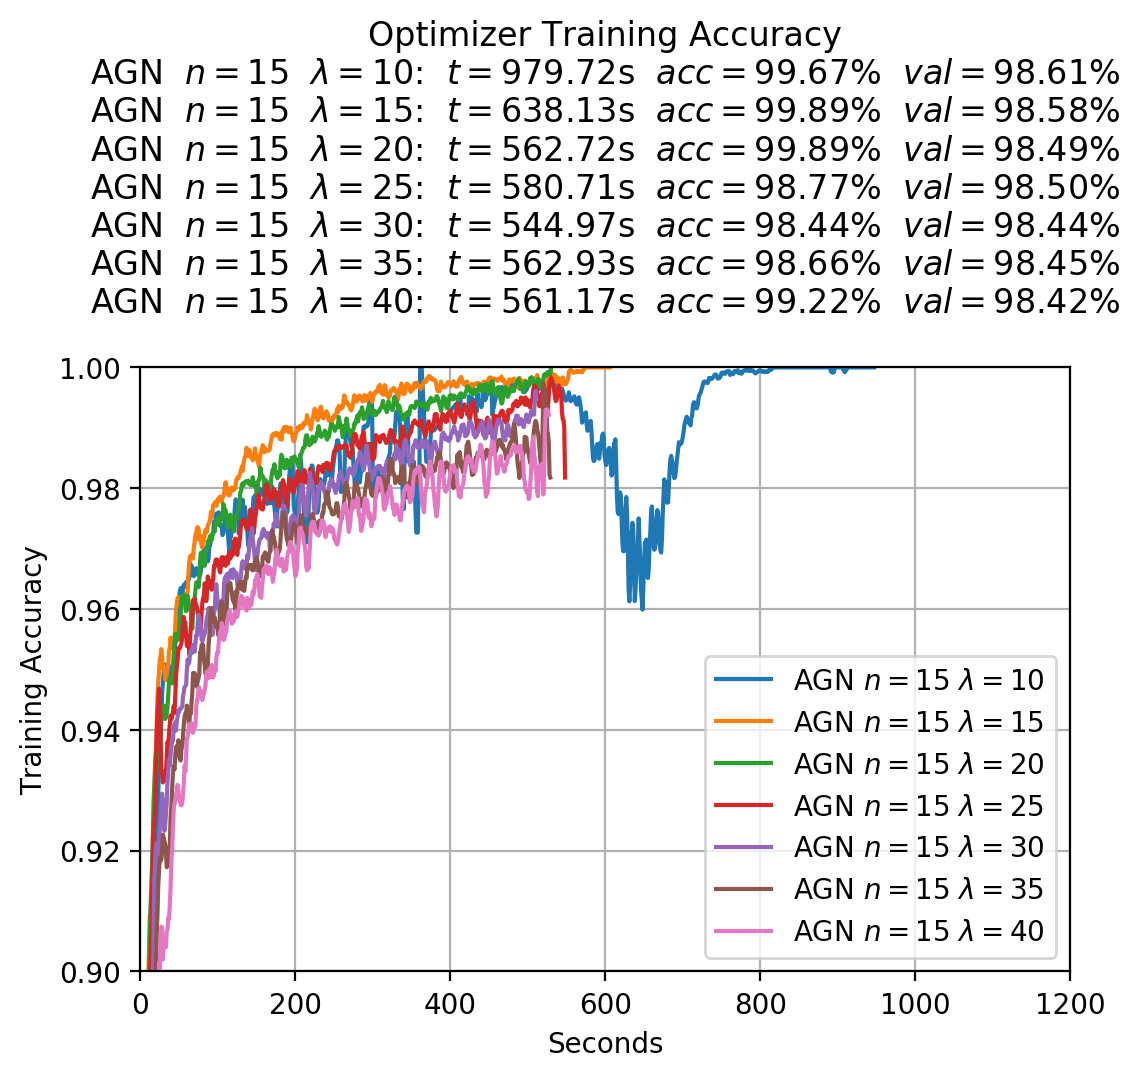
\includegraphics[width=\linewidth]{resources/images/agn_experiments_workers_15}
    \caption{$n = 15$}
  \end{subfigure}
  \begin{subfigure}{.3\textwidth}
    \centering
    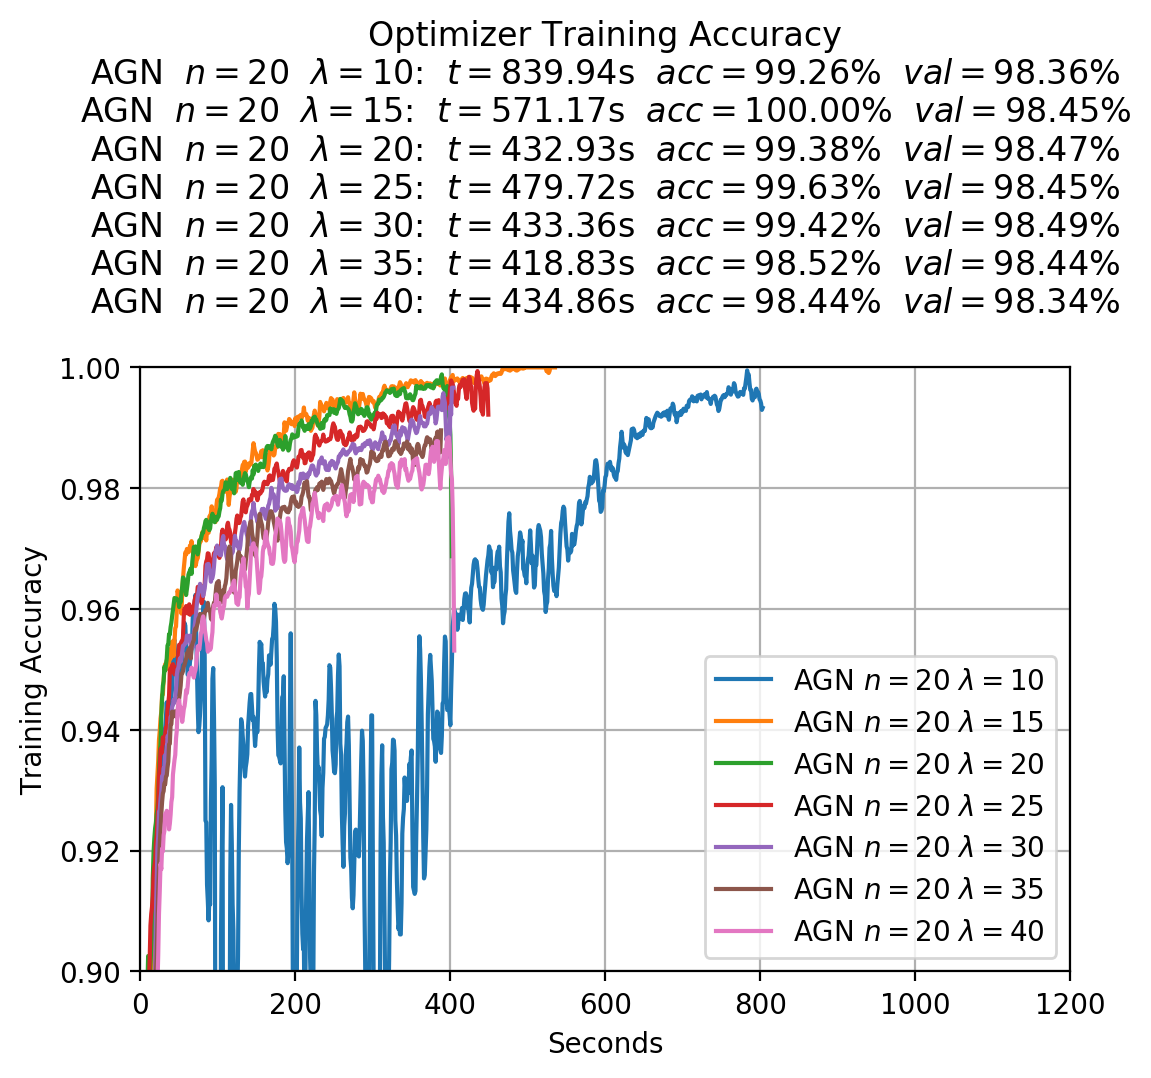
\includegraphics[width=\linewidth]{resources/images/agn_experiments_workers_20}
    \caption{$n = 20$}
  \end{subfigure}
  \begin{subfigure}{.3\textwidth}
    \centering
    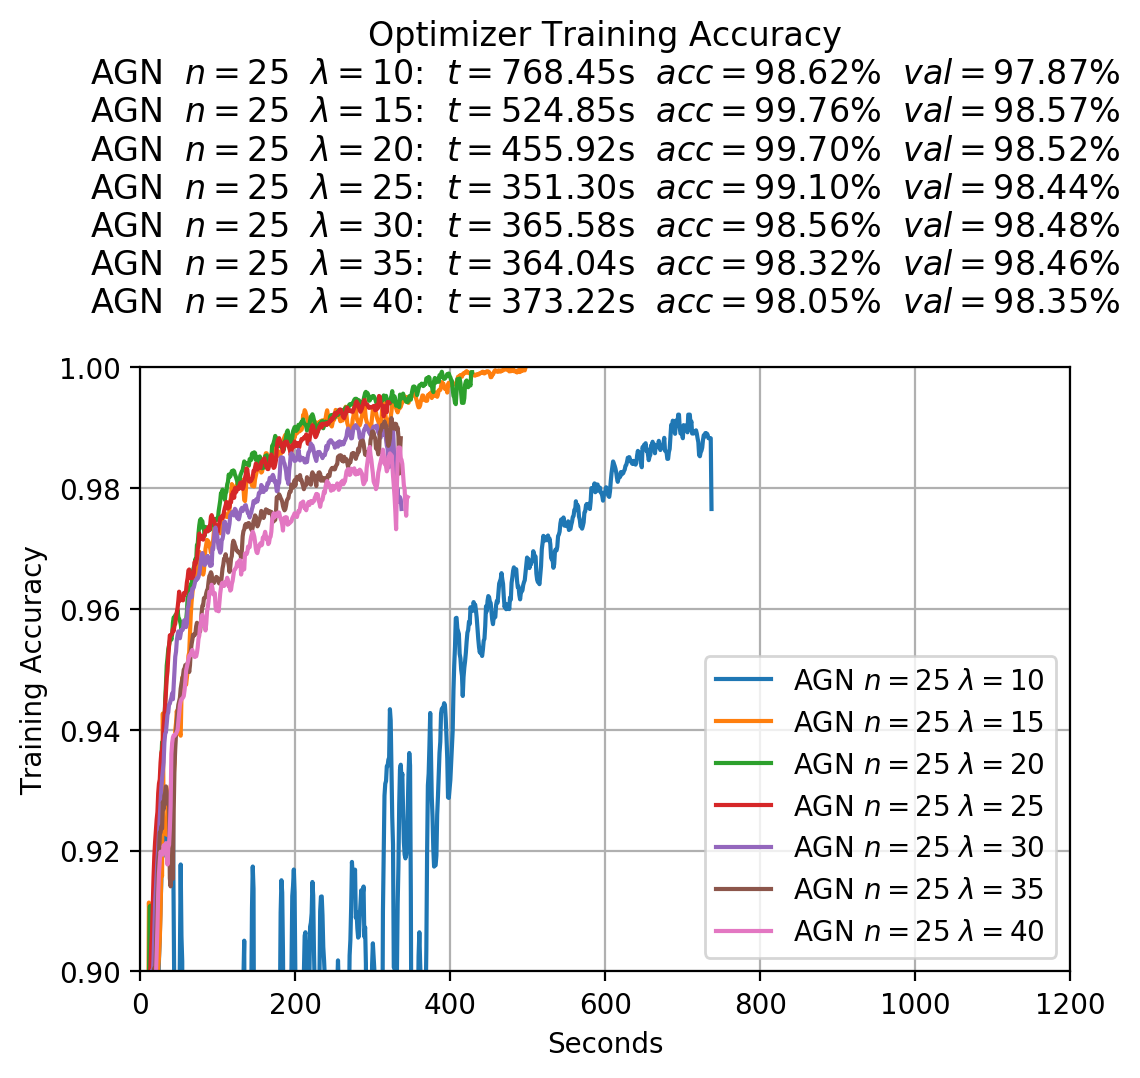
\includegraphics[width=\linewidth]{resources/images/agn_experiments_workers_25}
    \caption{$n = 25$}
  \end{subfigure}
  \begin{subfigure}{.3\textwidth}
    \centering
    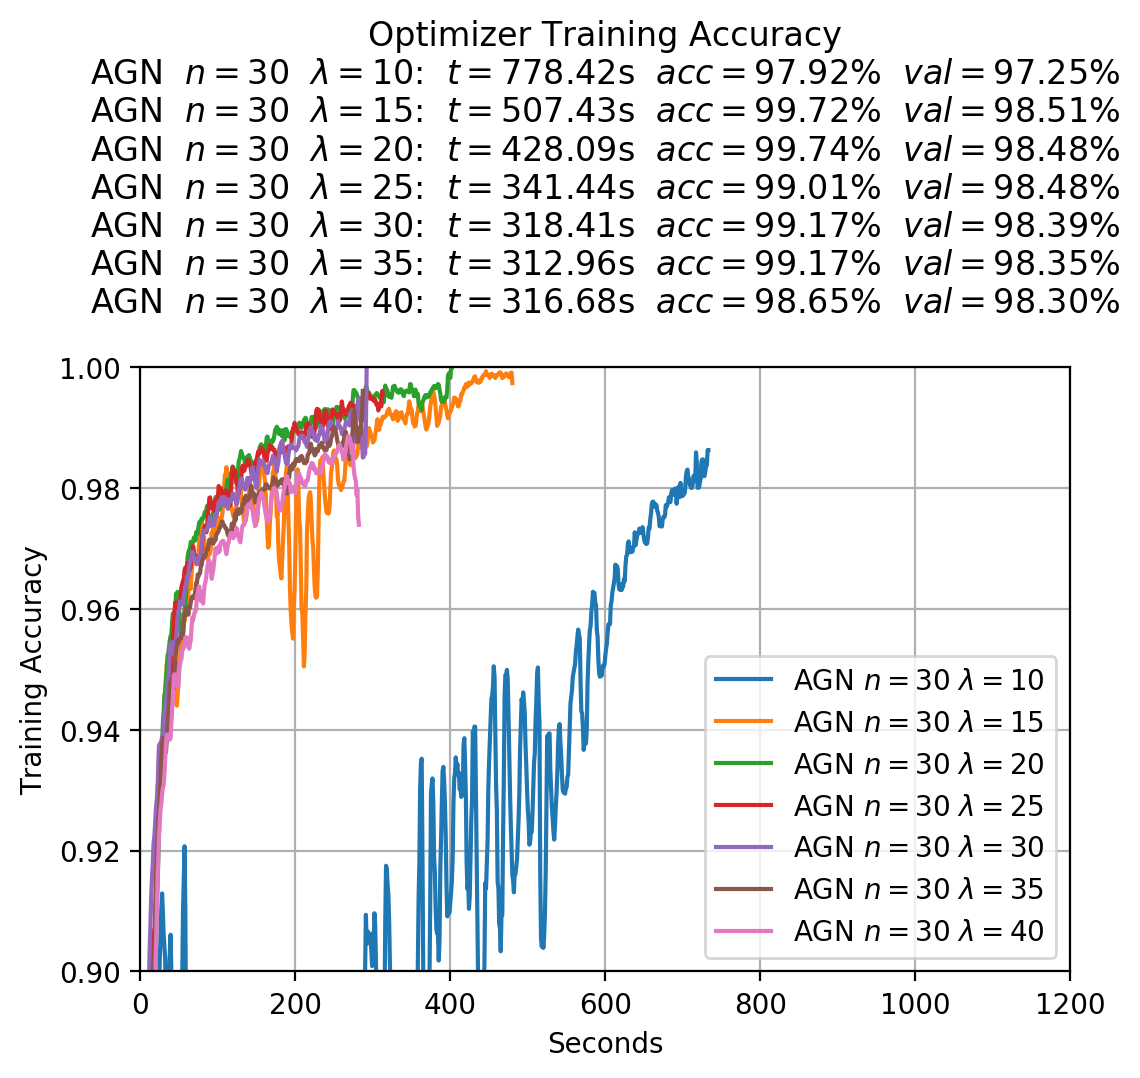
\includegraphics[width=\linewidth]{resources/images/agn_experiments_workers_30}
    \caption{$n = 30$}
  \end{subfigure}
  \begin{subfigure}{.3\textwidth}
    \centering
    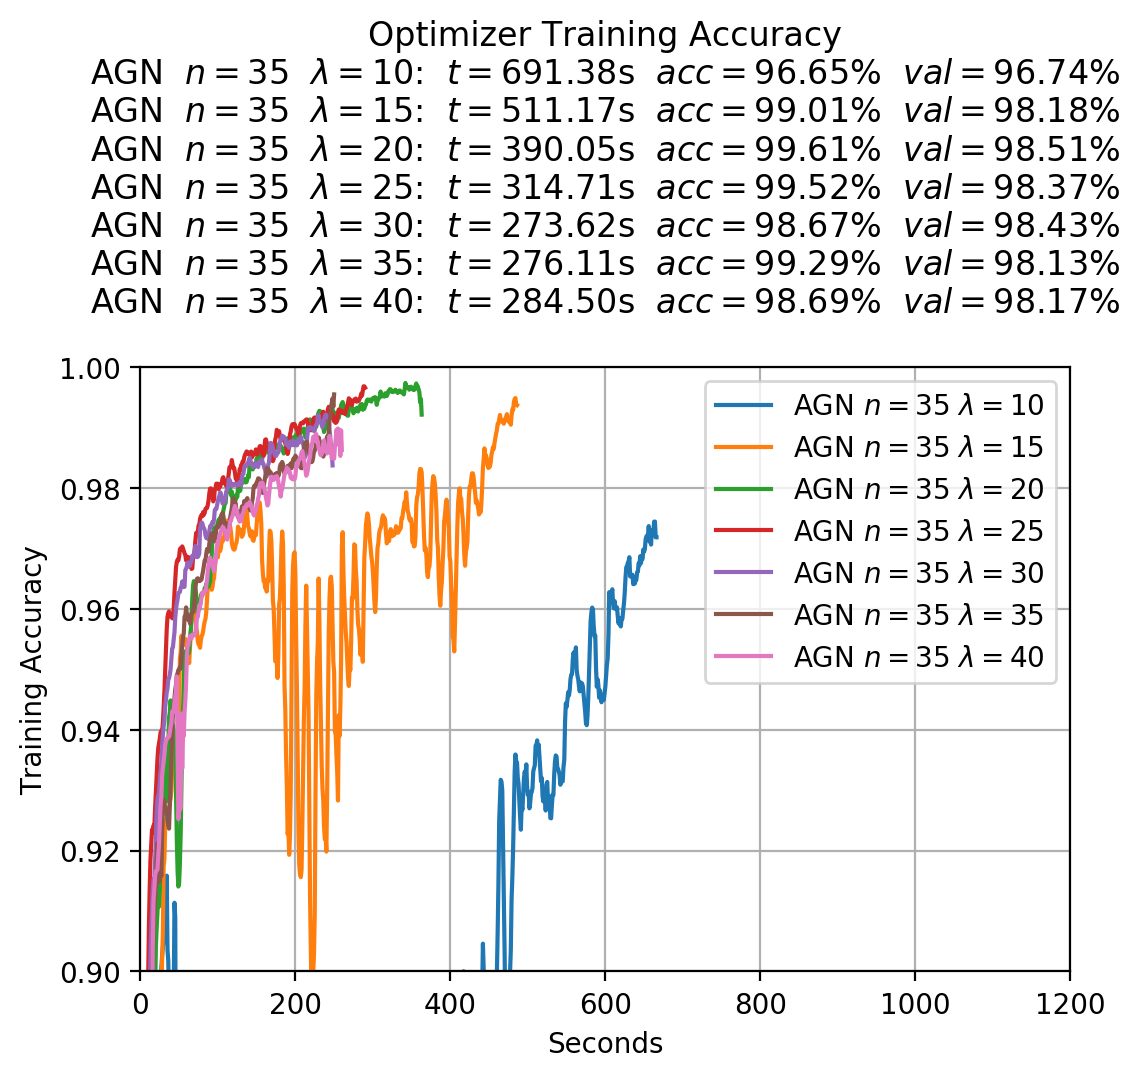
\includegraphics[width=\linewidth]{resources/images/agn_experiments_workers_35}
    \caption{$n = 35$}
  \end{subfigure}
  \begin{subfigure}{.3\textwidth}
    \centering
    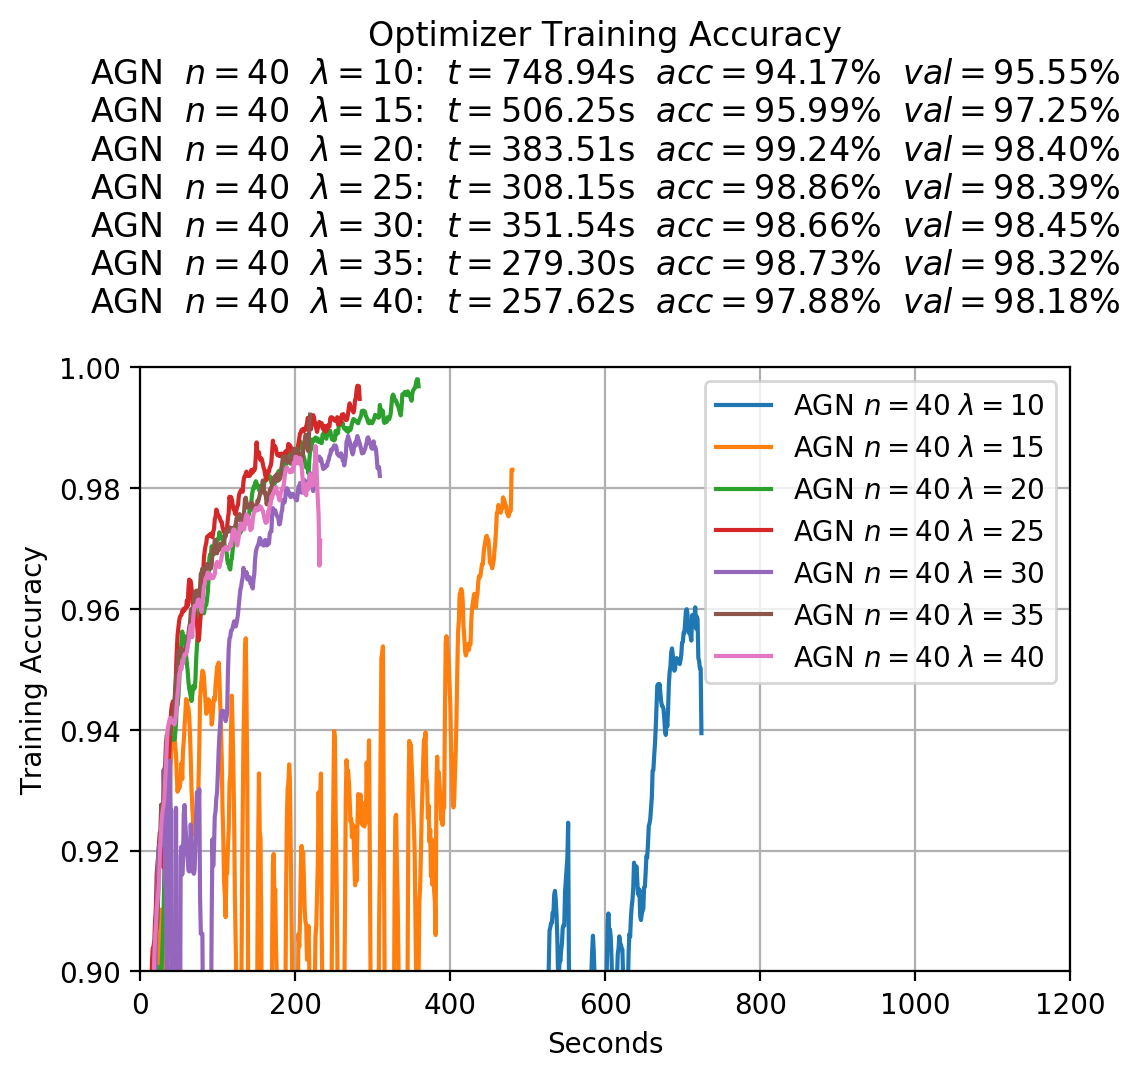
\includegraphics[width=\linewidth]{resources/images/agn_experiments_workers_40}
    \caption{$n = 40$}
  \end{subfigure}
  \caption{This Figure shows several experiments were we fixed the number of workers, but vary the communication frequency. From this we observe that \textsc{agn} performs well when a relatively equal high communication frequency is used with respect to the number of workers, and derrive the following heuristic $\lambda \approx \frac{n + \text{layers in network}}{2}$. Furthermore, increasing the amount of workers, and maintaining a high communication frequency deteriorates the performance of the central variable as well. As a result, a balance between the communication frequency, and the number of asynchronous workers is required.}
  \label{fig:agn_experiments_workers}
\end{figure}

\begin{figure}
  \centering
  \begin{subfigure}{.3\textwidth}
    \centering
    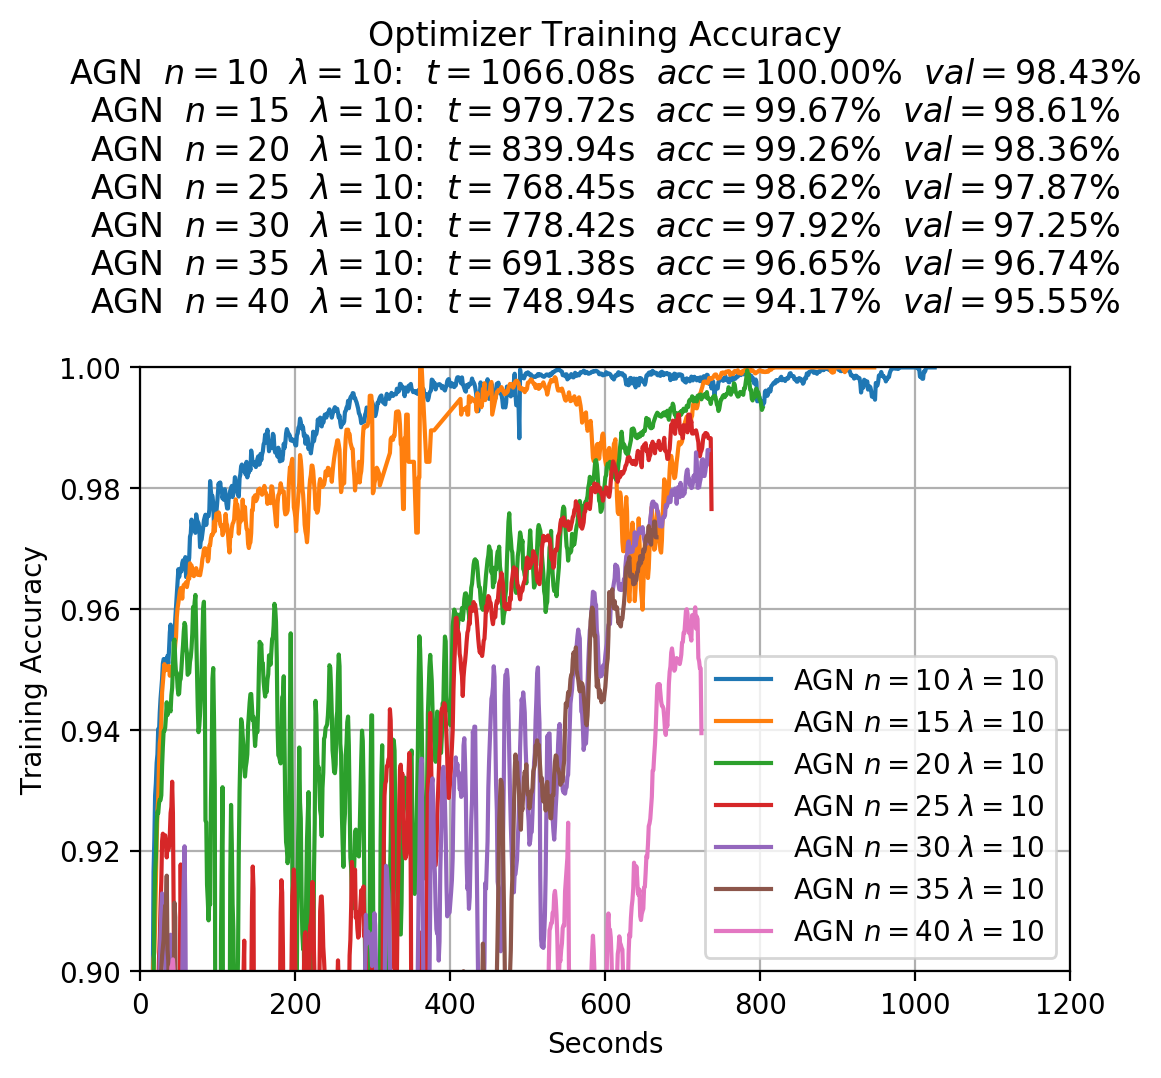
\includegraphics[width=\linewidth]{resources/images/agn_experiments_lambda_10}
    \caption{$\lambda = 10$}
  \end{subfigure}
  \begin{subfigure}{.3\textwidth}
    \centering
    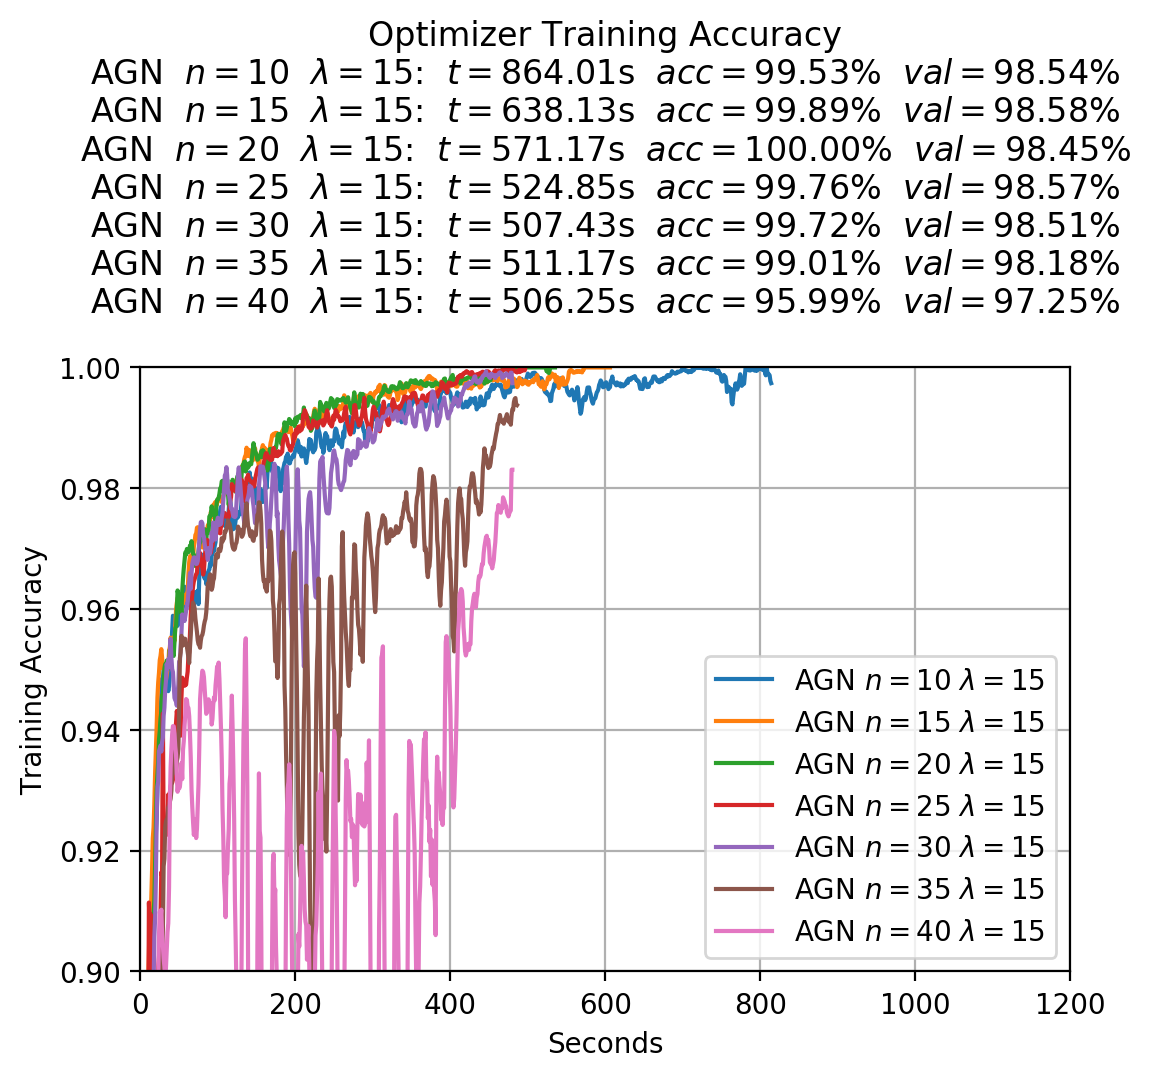
\includegraphics[width=\linewidth]{resources/images/agn_experiments_lambda_15}
    \caption{$\lambda = 15$}
  \end{subfigure}
  \begin{subfigure}{.3\textwidth}
    \centering
    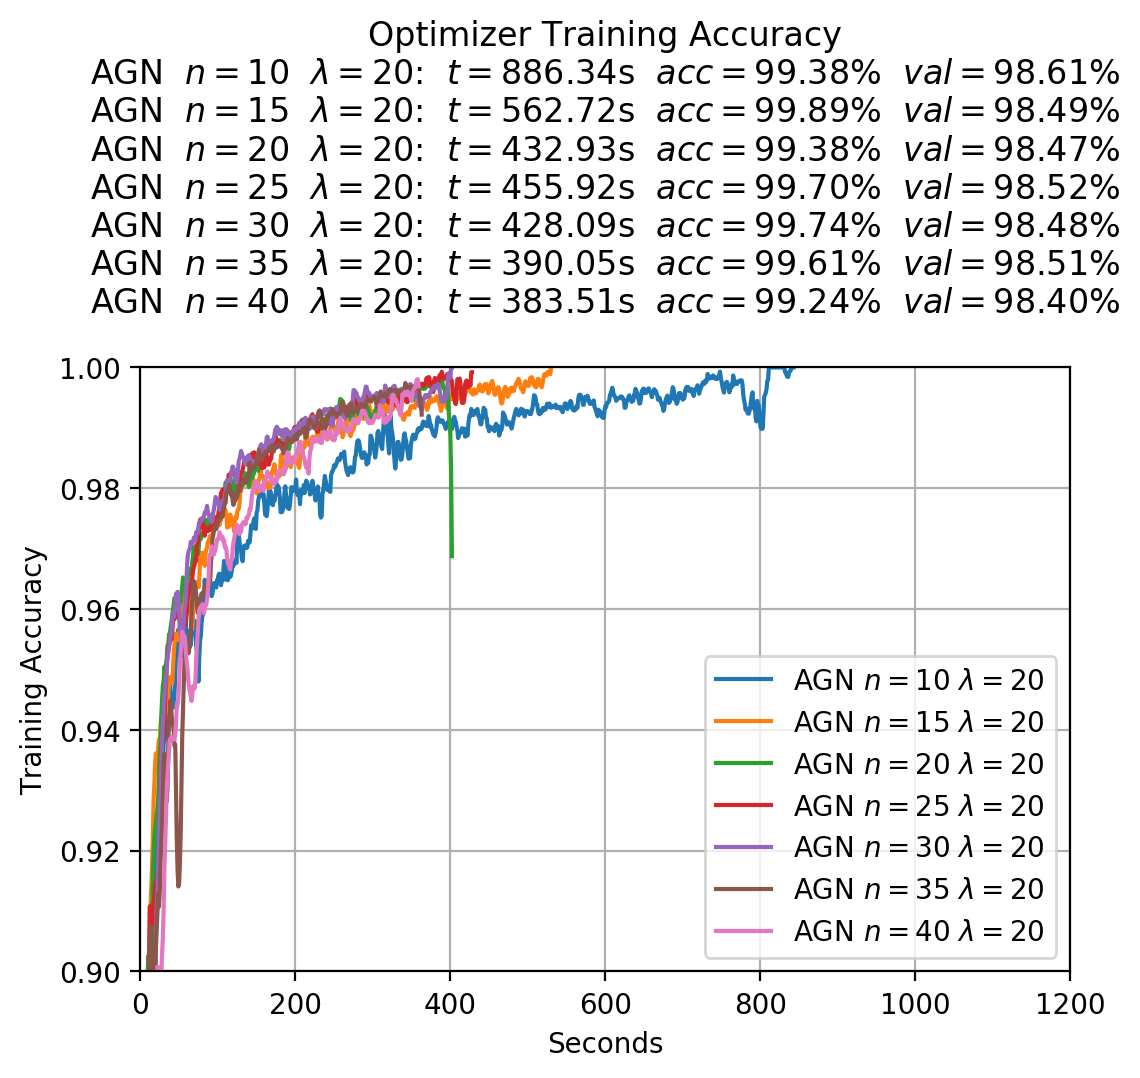
\includegraphics[width=\linewidth]{resources/images/agn_experiments_lambda_20}
    \caption{$\lambda = 20$}
  \end{subfigure}
  \begin{subfigure}{.3\textwidth}
    \centering
    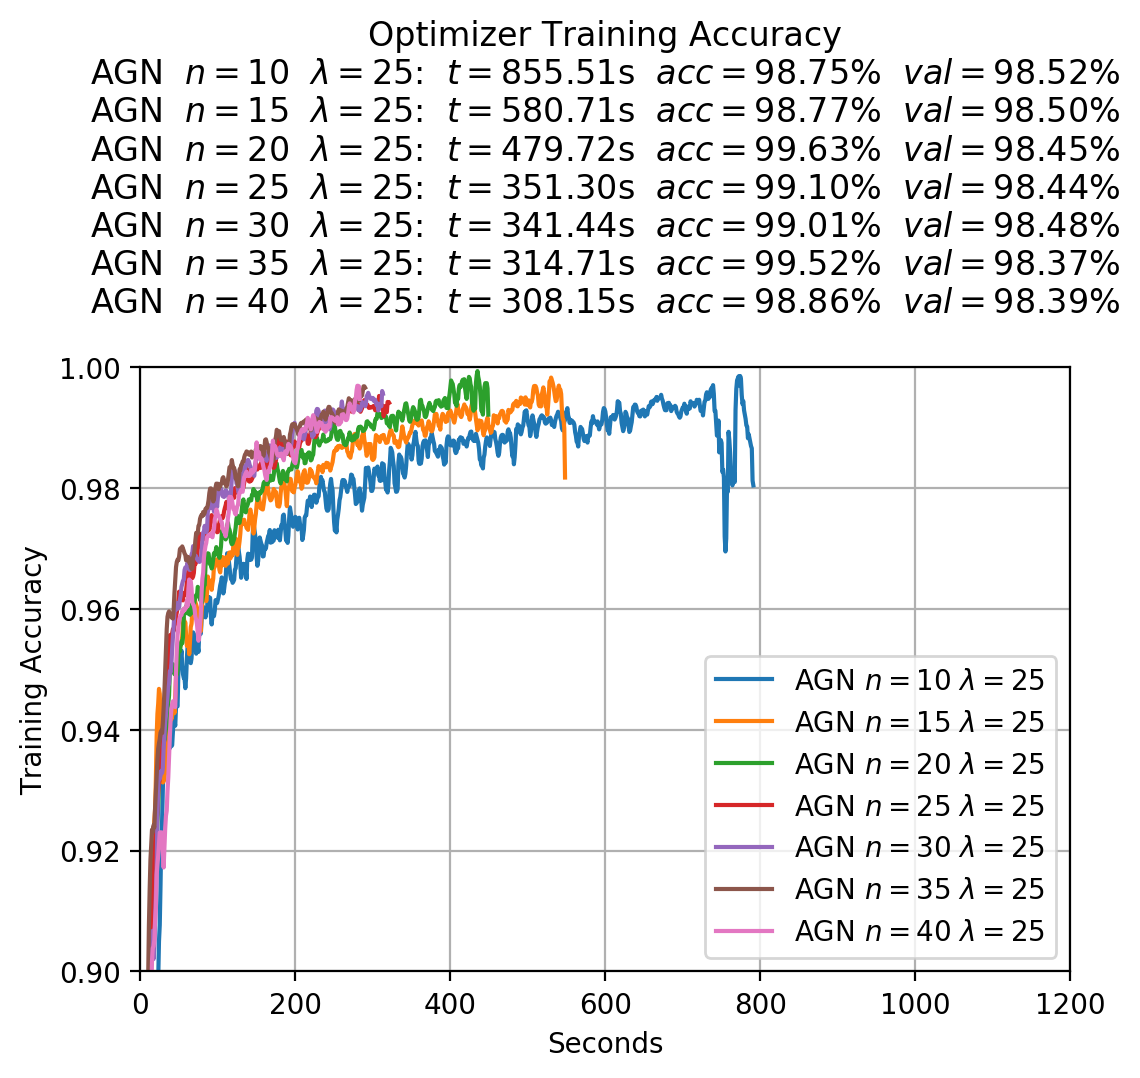
\includegraphics[width=\linewidth]{resources/images/agn_experiments_lambda_25}
    \caption{$\lambda = 25$}
  \end{subfigure}
  \begin{subfigure}{.3\textwidth}
    \centering
    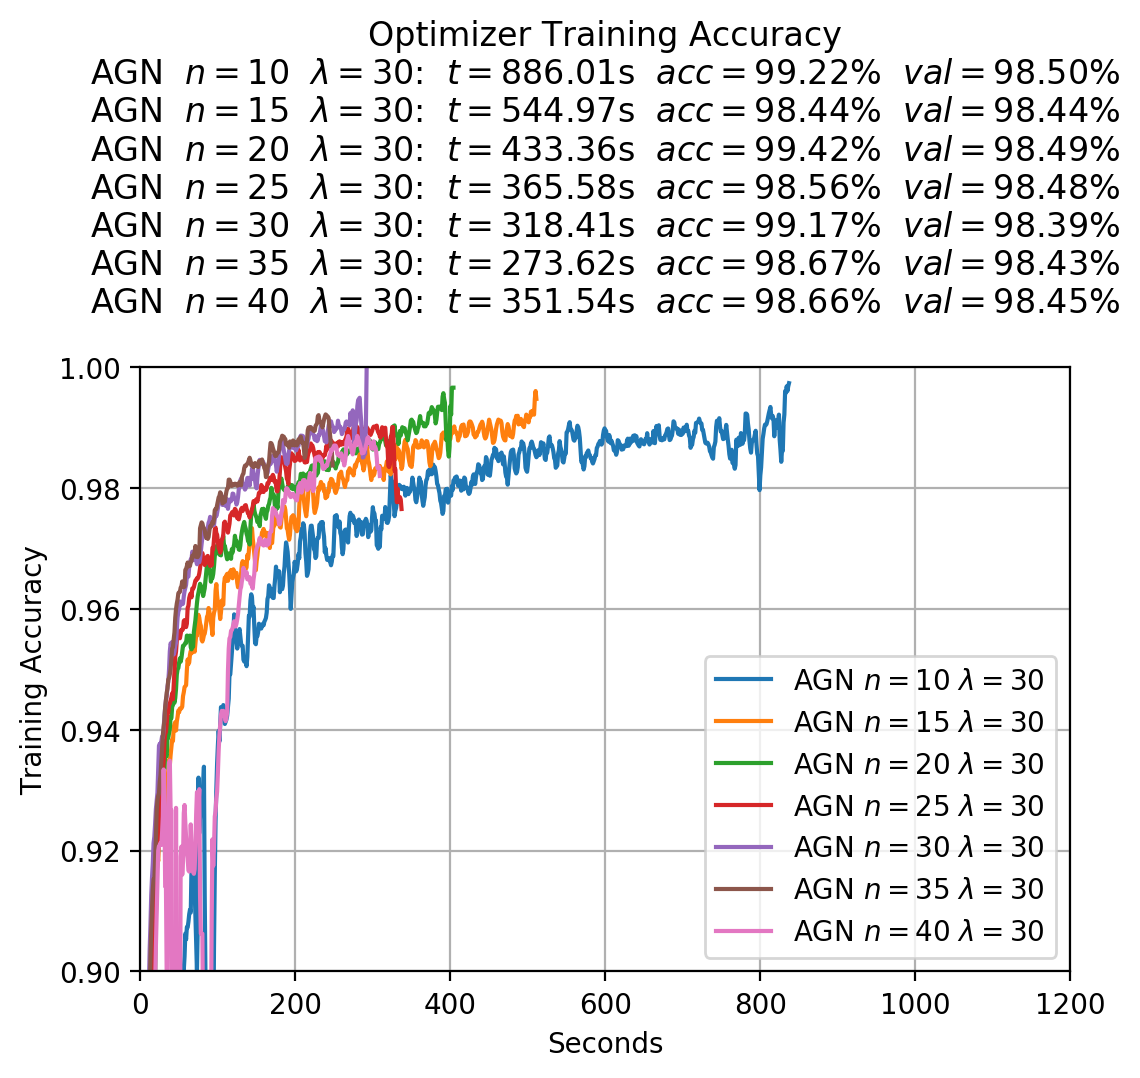
\includegraphics[width=\linewidth]{resources/images/agn_experiments_lambda_30}
    \caption{$\lambda = 30$}
  \end{subfigure}
  \begin{subfigure}{.3\textwidth}
    \centering
    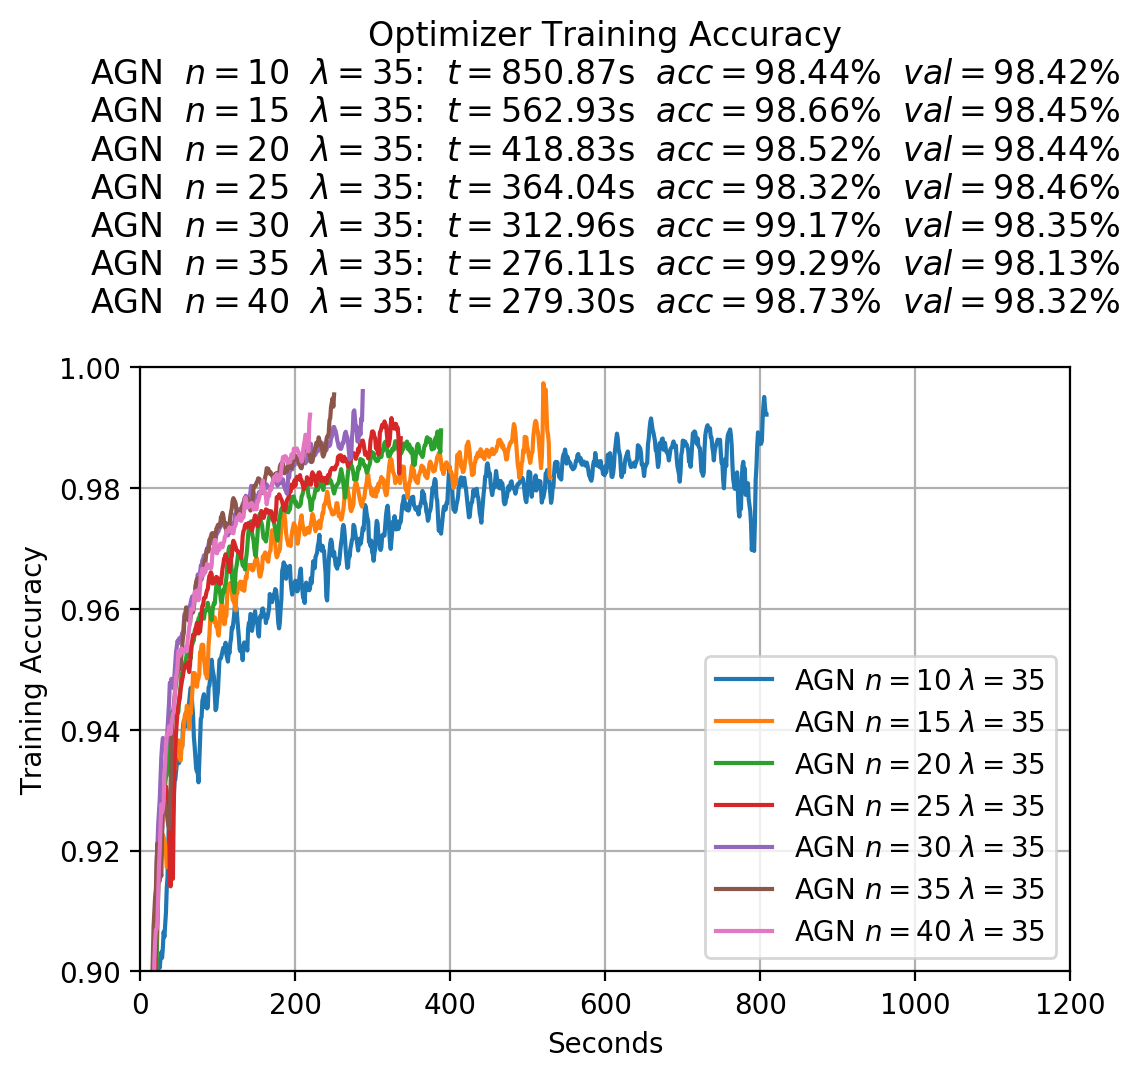
\includegraphics[width=\linewidth]{resources/images/agn_experiments_lambda_35}
    \caption{$\lambda = 35$}
  \end{subfigure}
  \begin{subfigure}{.3\textwidth}
    \centering
    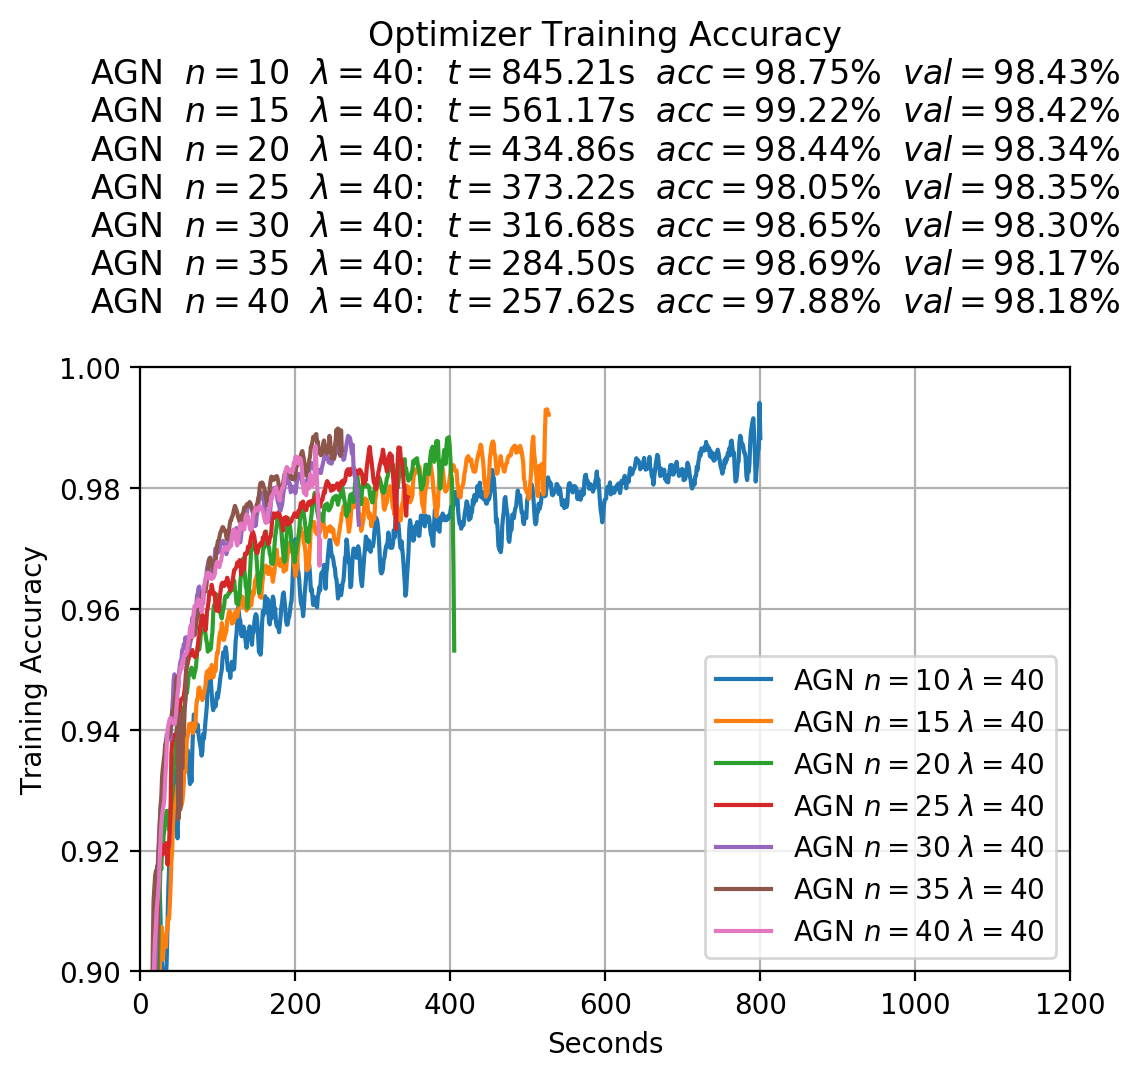
\includegraphics[width=\linewidth]{resources/images/agn_experiments_lambda_40}
    \caption{$\lambda = 40$}
  \end{subfigure}
  \caption{In this experiment we clamp the communication frequency, but vary the number of asynchronous workers. Due to the equal communication frequency, we can observe good scaling properties of \textsc{agn}. In most cases doubling the number of workers, reducing the training time by half and is more temporally efficient. However, for larger number of workers $n > 30$ we do not observe a reduction of training time. This is due to the implementation of our parameter server, which is based on Python threads instead of Python processes, as will be dicussed in Chapter~\ref{chapter:experiments}. Furthermore, note that reducing the amount of computational resources might actually benifit the training accuracy of the central variable, as a smaller number of asynchronous workers reduces the amount of staleness that can be incorperated in the central variable.}
  \label{fig:agn_experiments_lambdas}
\end{figure}

\begin{figure}
  \centering
  \begin{subfigure}{.3\textwidth}
    \centering
    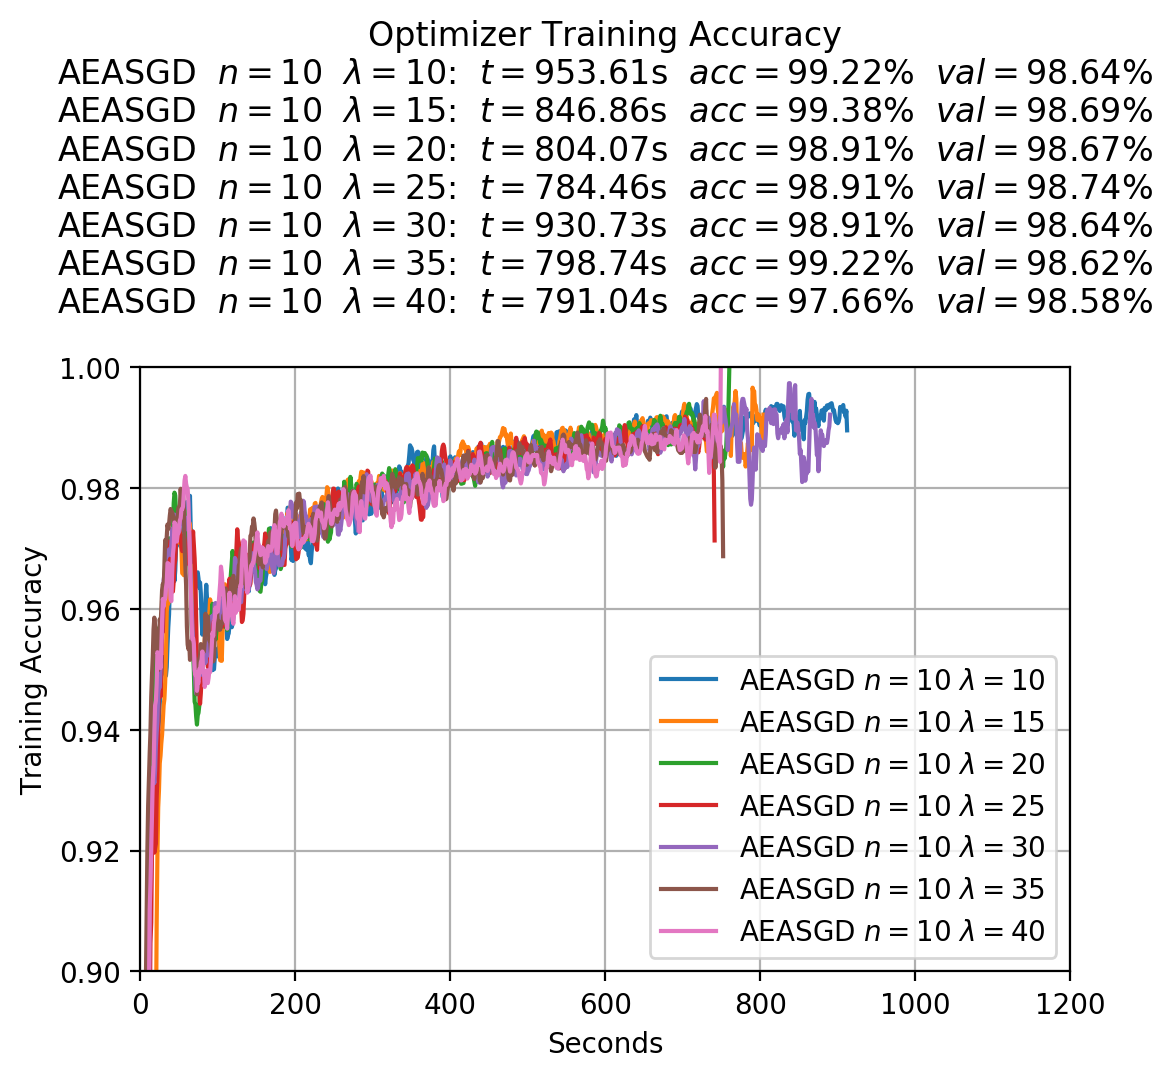
\includegraphics[width=\linewidth]{resources/images/aeasgd_experiments_workers_10}
    \caption{$n = 10$}
  \end{subfigure}
  \begin{subfigure}{.3\textwidth}
    \centering
    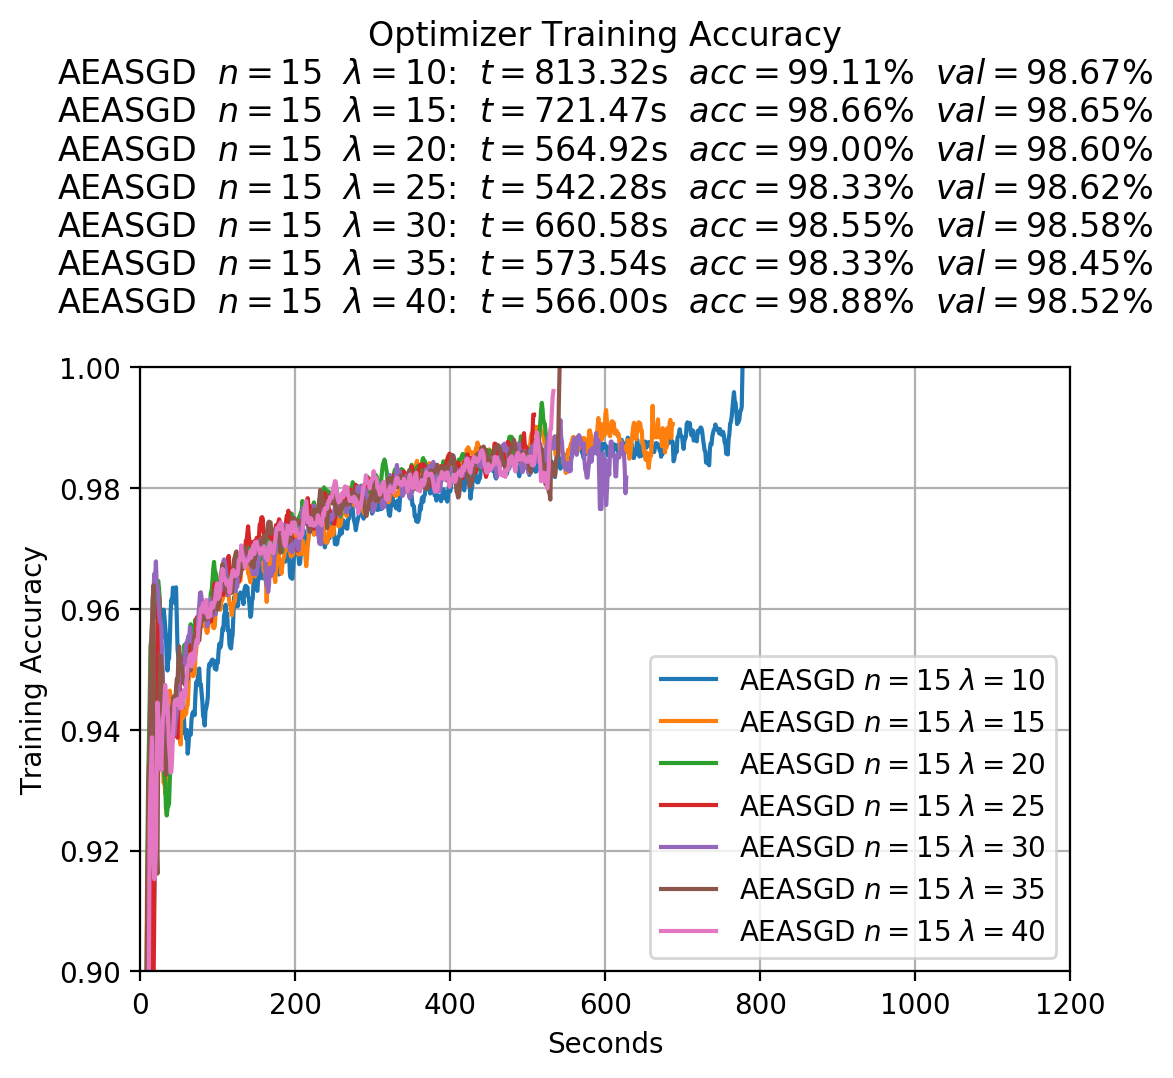
\includegraphics[width=\linewidth]{resources/images/aeasgd_experiments_workers_15}
    \caption{$n = 15$}
  \end{subfigure}
  \begin{subfigure}{.3\textwidth}
    \centering
    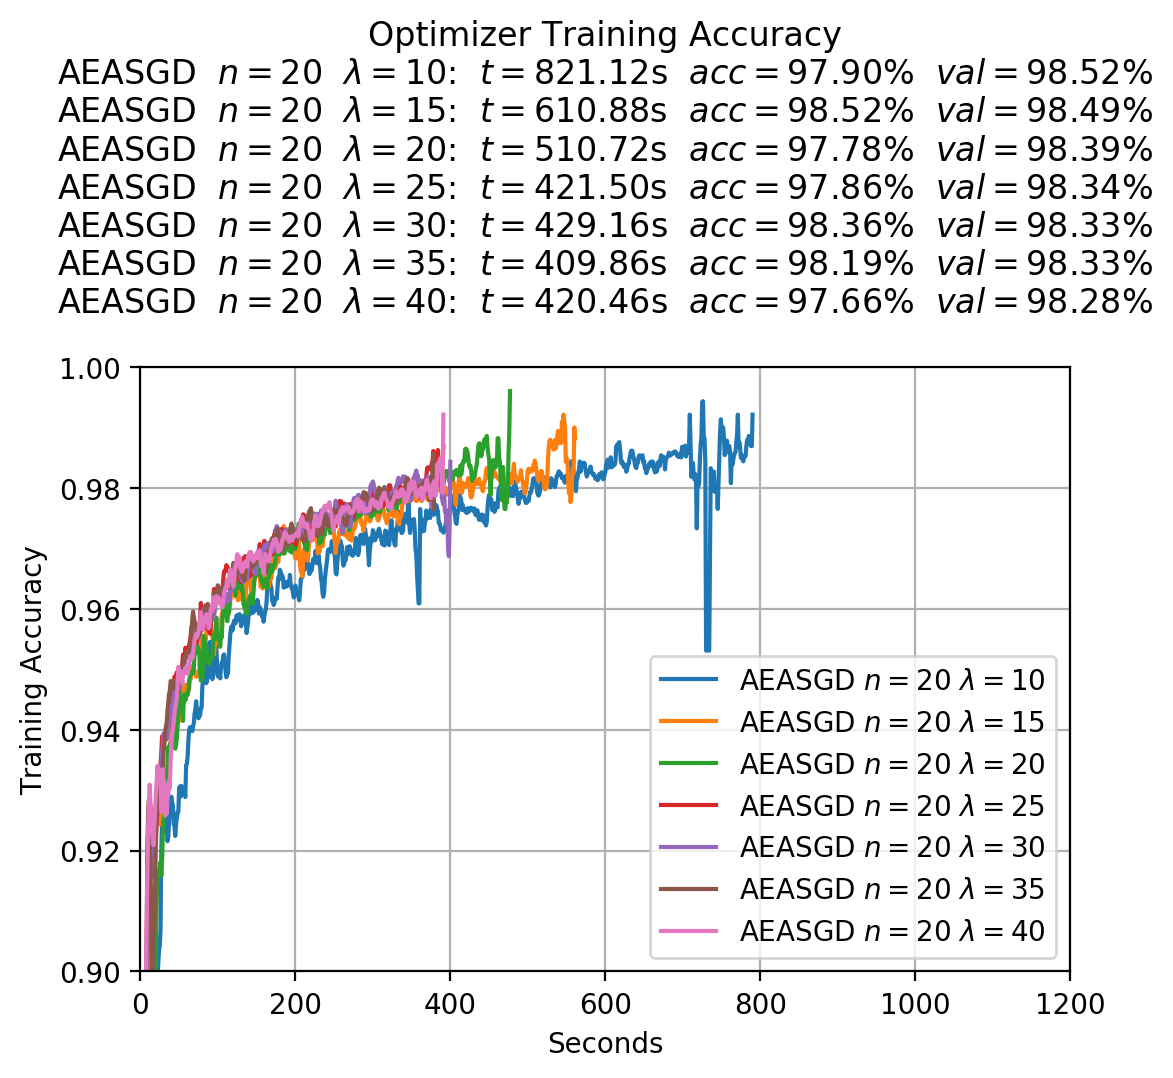
\includegraphics[width=\linewidth]{resources/images/aeasgd_experiments_workers_20}
    \caption{$n = 20$}
  \end{subfigure}
  \begin{subfigure}{.3\textwidth}
    \centering
    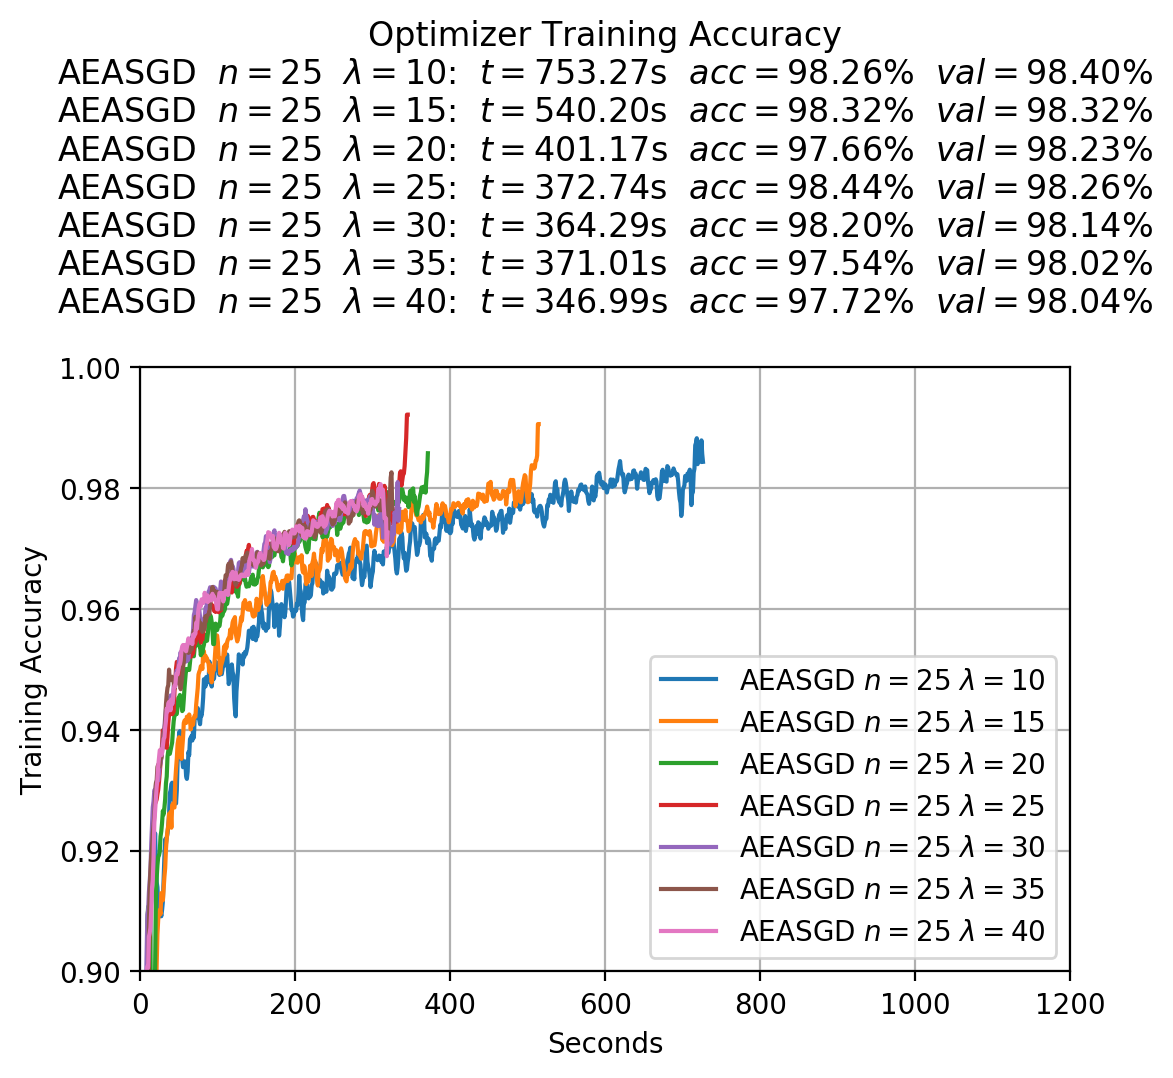
\includegraphics[width=\linewidth]{resources/images/aeasgd_experiments_workers_25}
    \caption{$n = 25$}
  \end{subfigure}
  \begin{subfigure}{.3\textwidth}
    \centering
    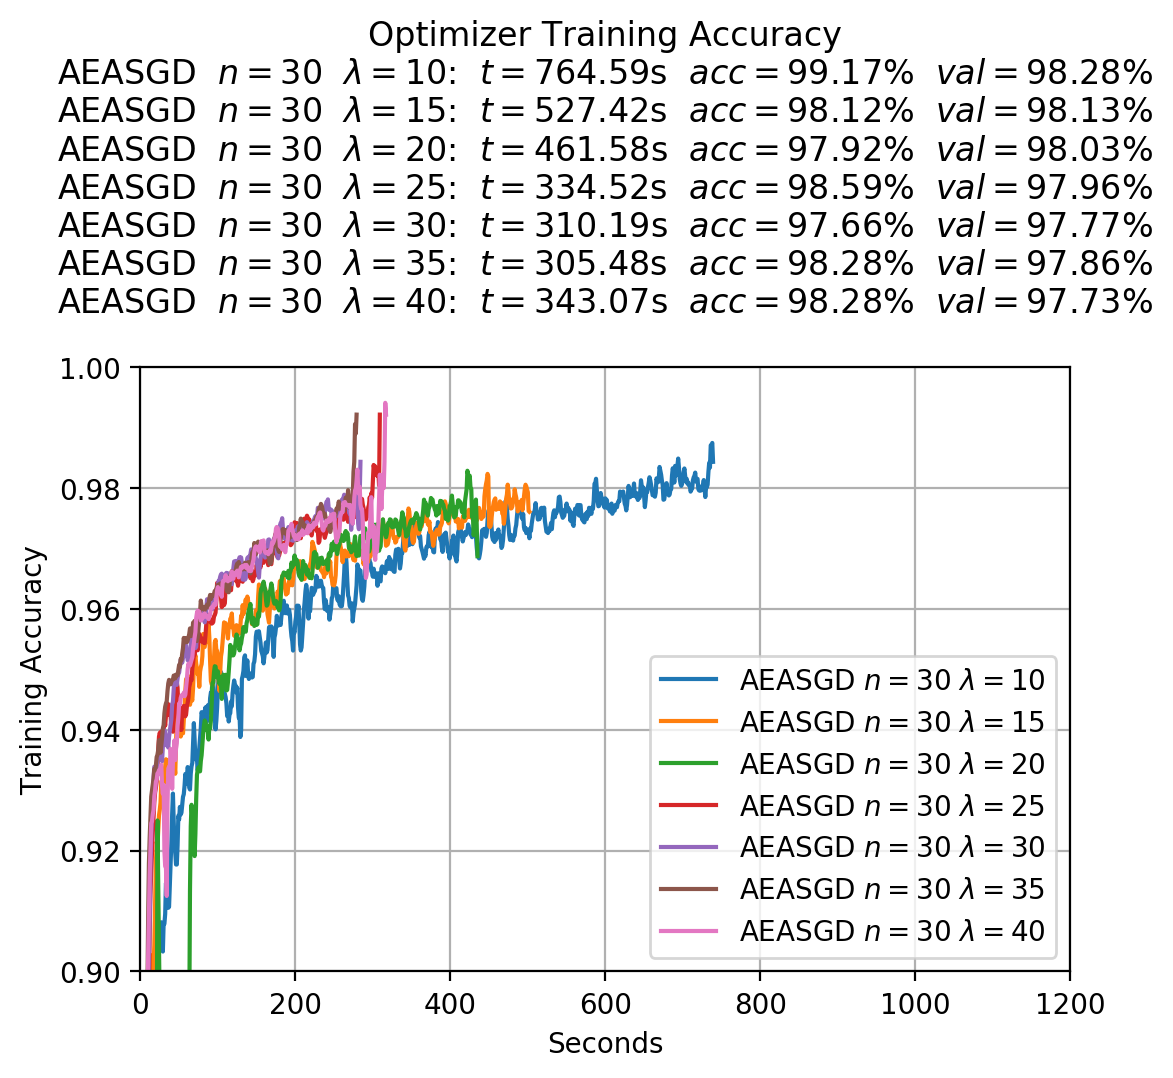
\includegraphics[width=\linewidth]{resources/images/aeasgd_experiments_workers_30}
    \caption{$n = 30$}
  \end{subfigure}
  \begin{subfigure}{.3\textwidth}
    \centering
    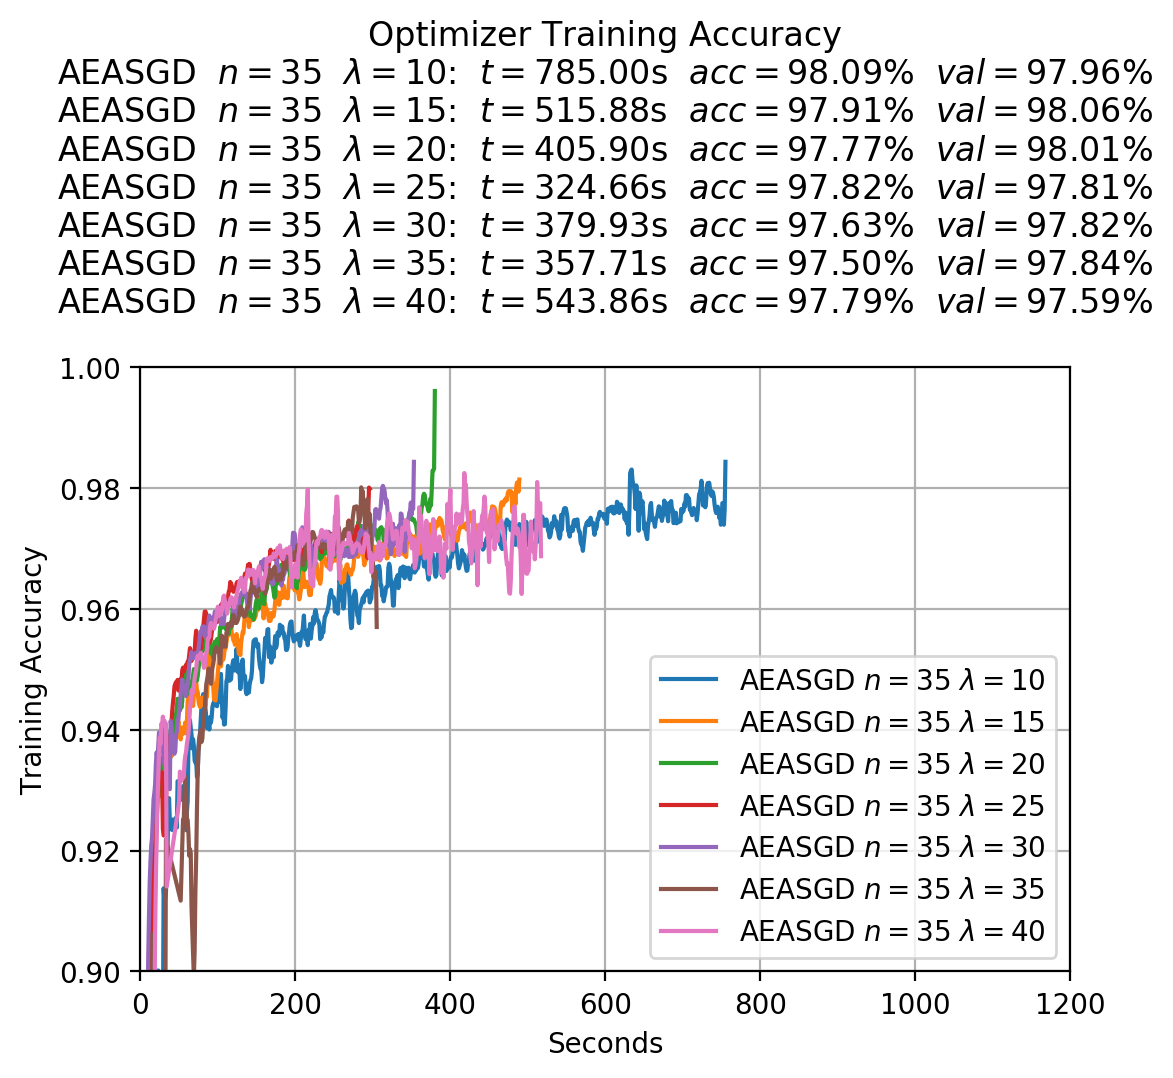
\includegraphics[width=\linewidth]{resources/images/aeasgd_experiments_workers_35}
    \caption{$n = 35$}
  \end{subfigure}
  \begin{subfigure}{.3\textwidth}
    \centering
    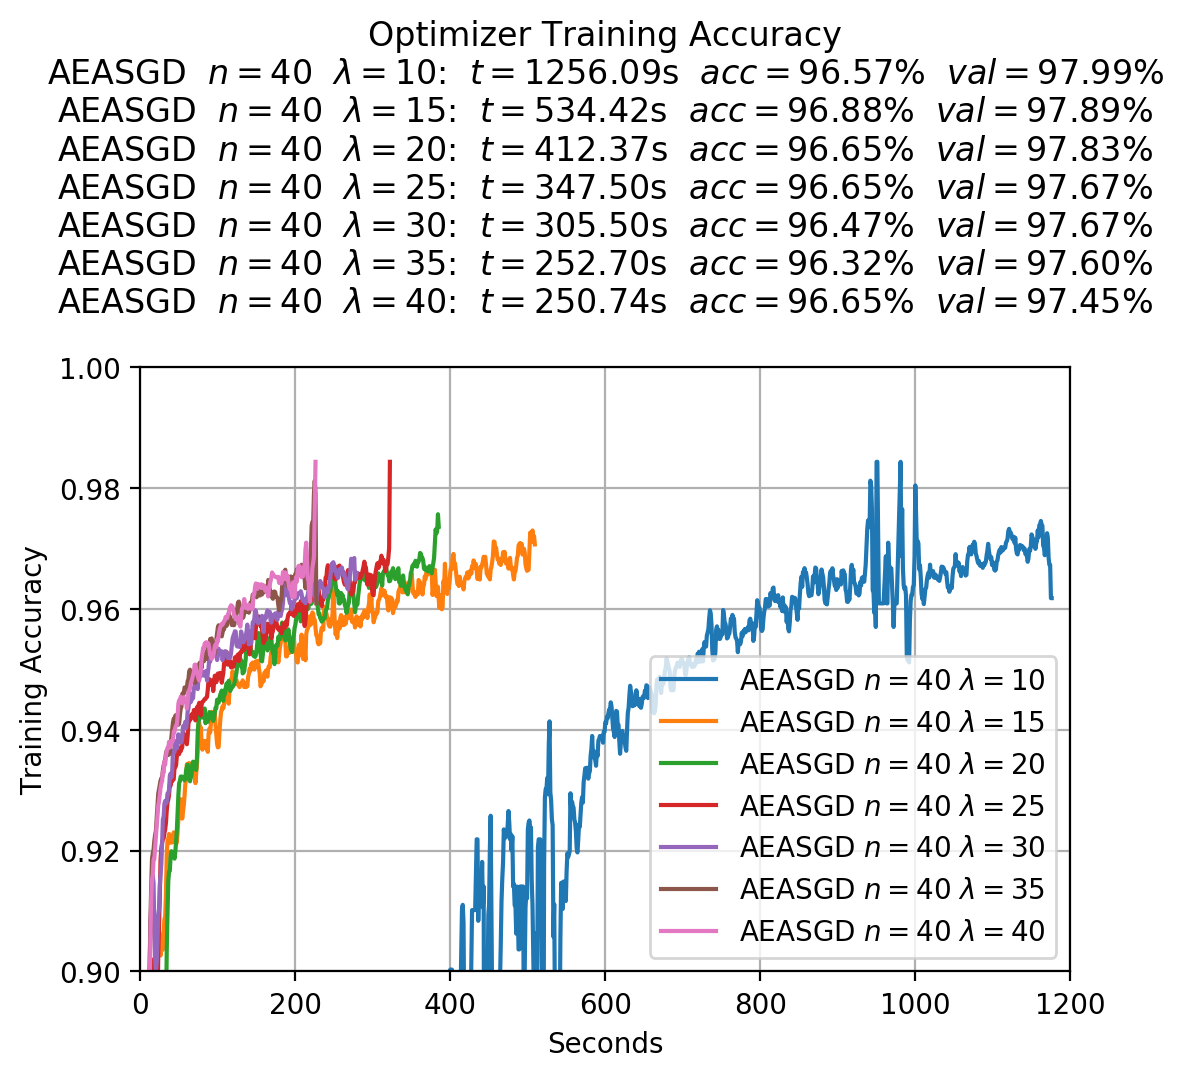
\includegraphics[width=\linewidth]{resources/images/aeasgd_experiments_workers_40}
    \caption{$n = 40$}
  \end{subfigure}
  \caption{\textsc{aeasgd} fixed worker, with varying communication frequency experiments. As suggested by the author, \textsc{aeasgd} usually benifits from an increased amount of local worker (large $\lambda$). Furthermore, we observe that initially, \textsc{aeasgd} is quite robust to hyperparameterization ($n = 10$). However, as the number of asynchronous workers increases, and the communication frequency is further reduced, the accuracy plots start to deviate to the point that they \emph{flatten} at a suboptimal training accuracy. Meaning, a lower training accuracy compared to other configurations, where \textsc{aeasgd} reached a significantly higher training accuracy.}
  \label{fig:aeasgd_experiments_workers}
\end{figure}

\begin{figure}
  \centering
  \begin{subfigure}{.3\textwidth}
    \centering
    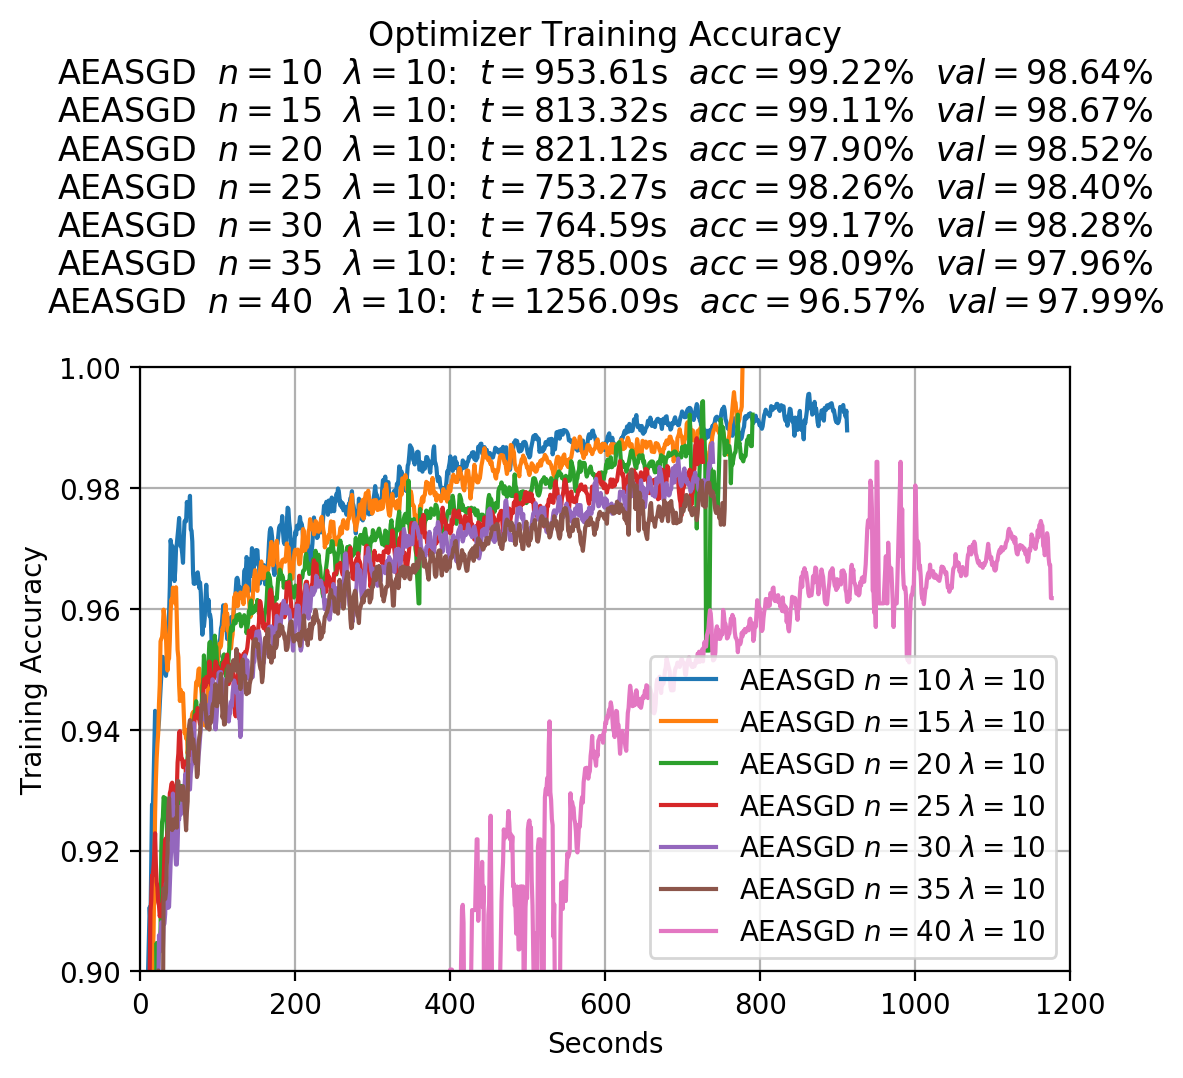
\includegraphics[width=\linewidth]{resources/images/aeasgd_experiments_lambda_10}
    \caption{$\lambda = 10$}
  \end{subfigure}
  \begin{subfigure}{.3\textwidth}
    \centering
    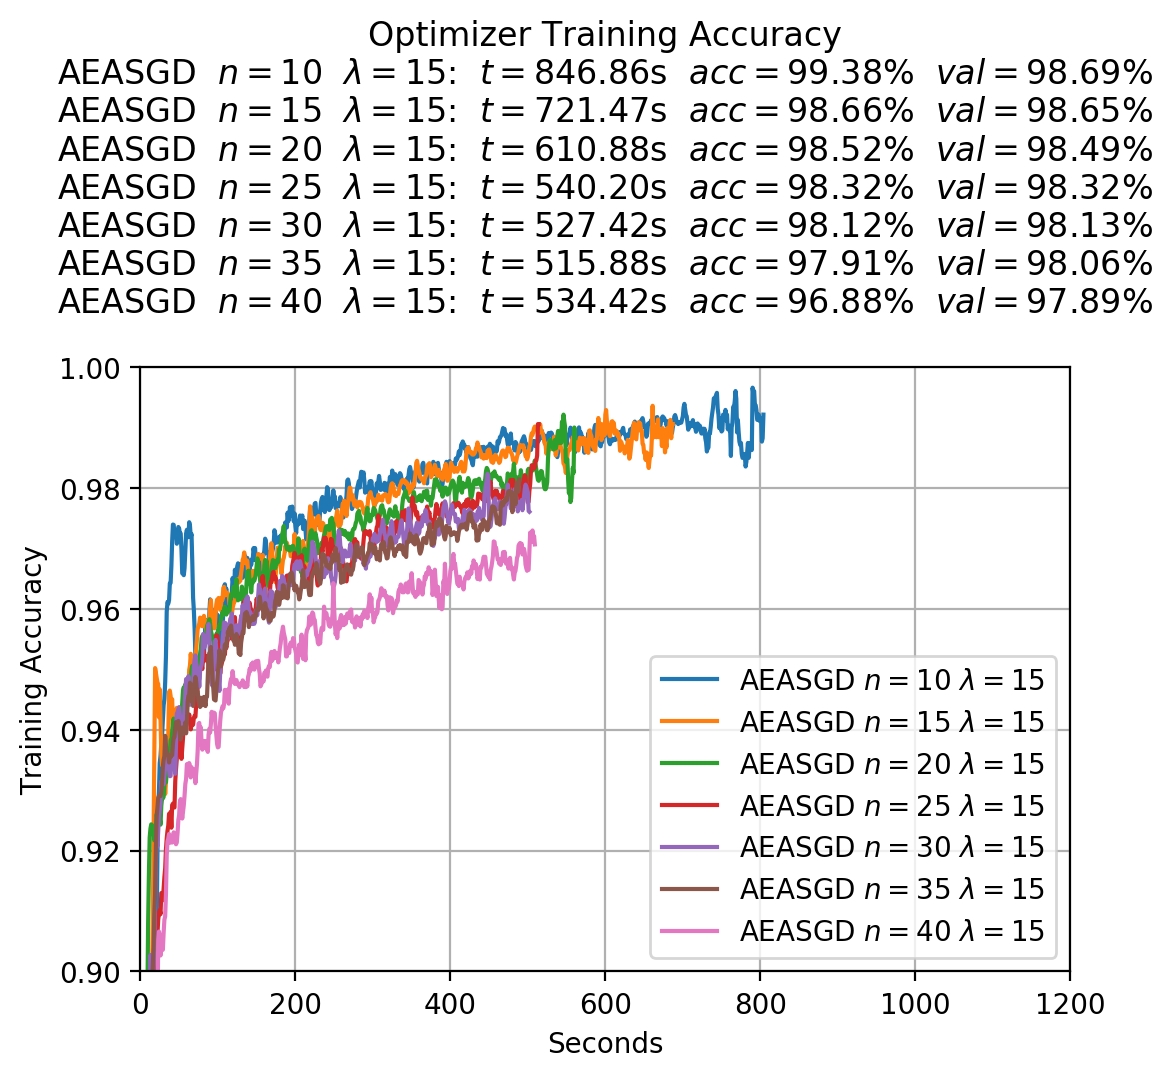
\includegraphics[width=\linewidth]{resources/images/aeasgd_experiments_lambda_15}
    \caption{$\lambda = 15$}
  \end{subfigure}
  \begin{subfigure}{.3\textwidth}
    \centering
    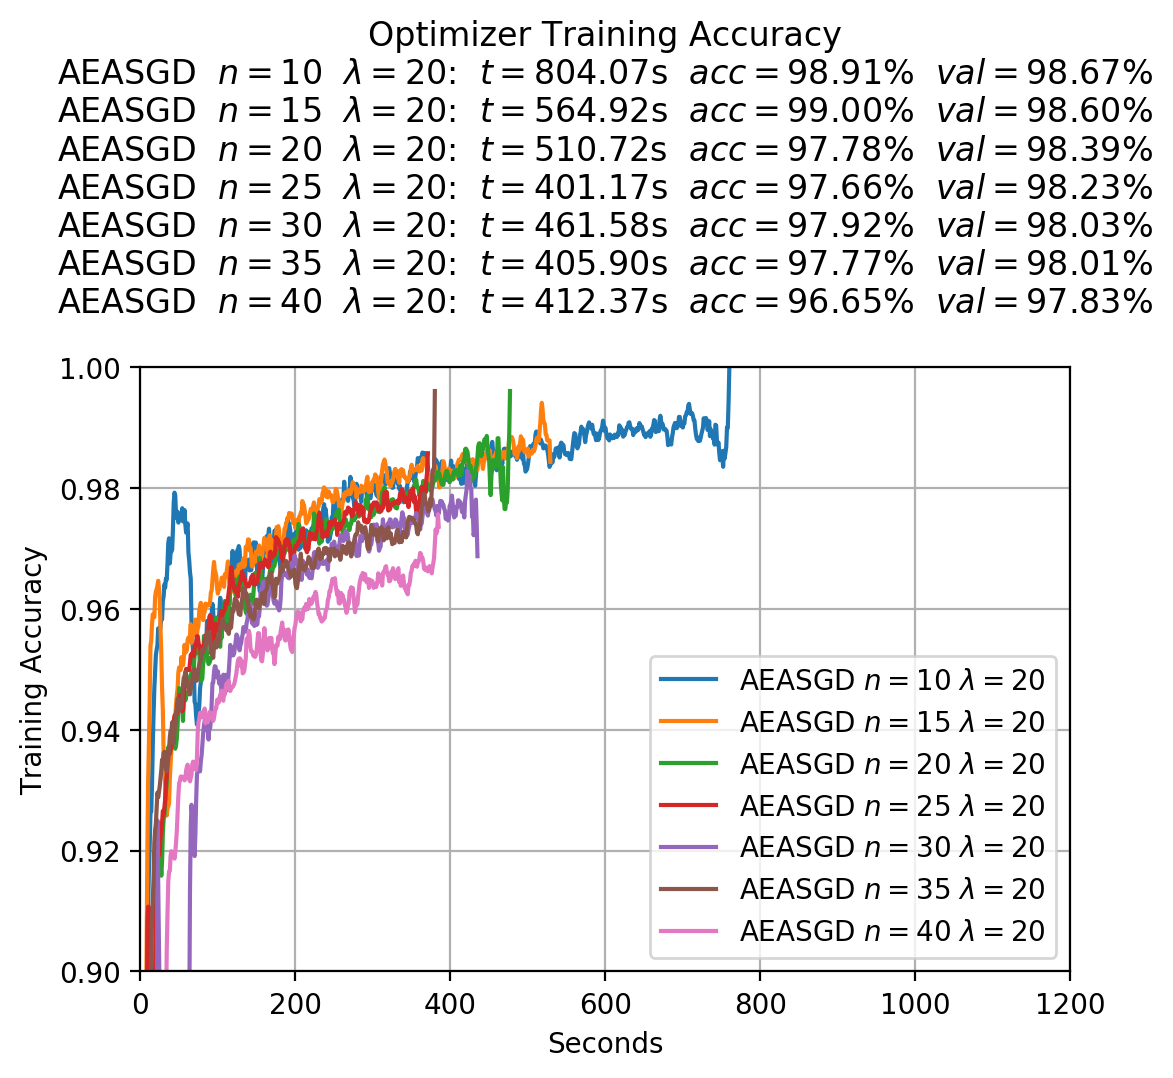
\includegraphics[width=\linewidth]{resources/images/aeasgd_experiments_lambda_20}
    \caption{$\lambda = 20$}
  \end{subfigure}
  \begin{subfigure}{.3\textwidth}
    \centering
    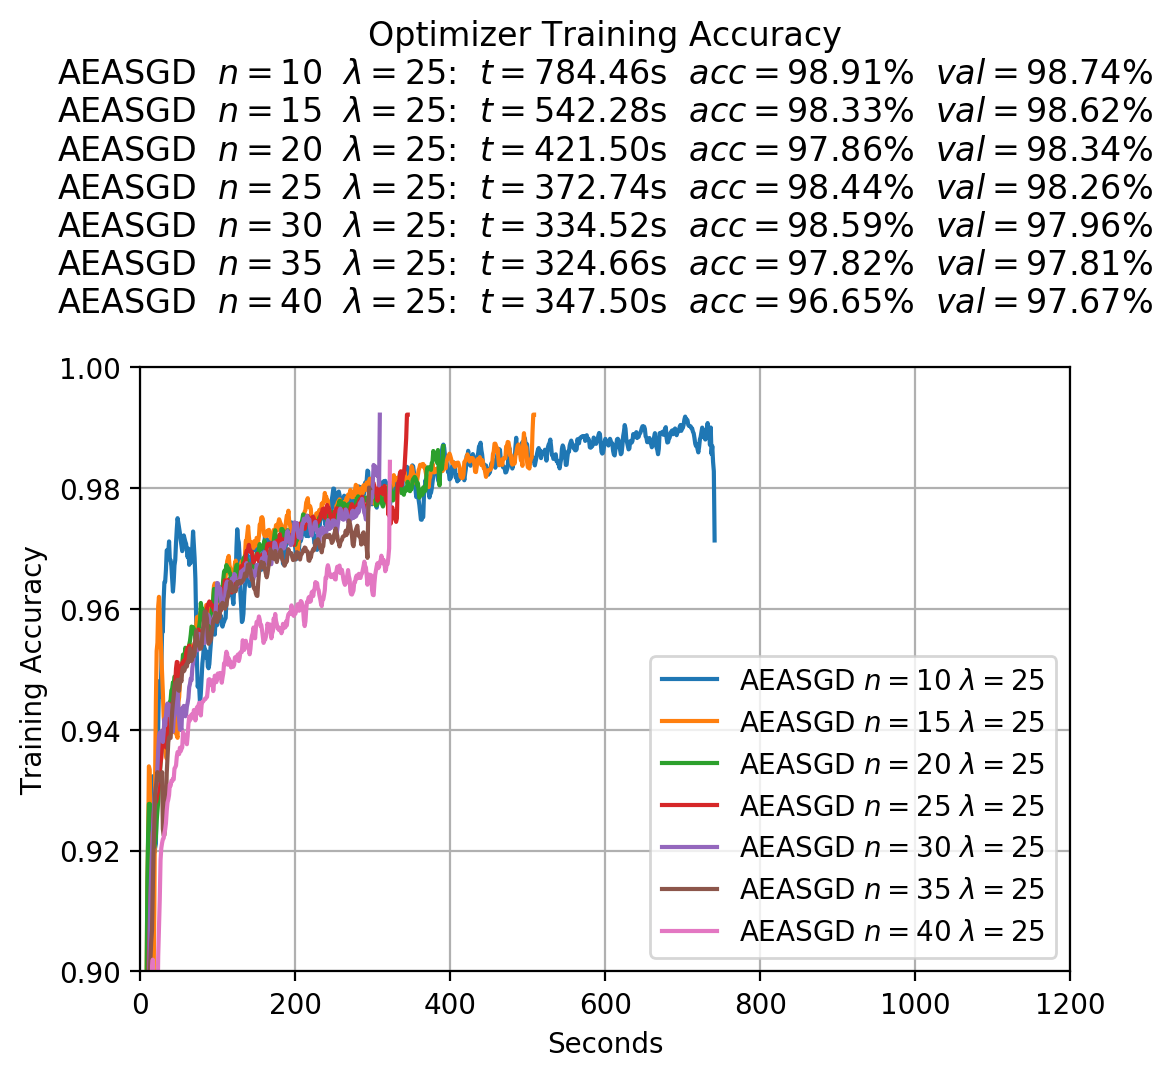
\includegraphics[width=\linewidth]{resources/images/aeasgd_experiments_lambda_25}
    \caption{$\lambda = 25$}
  \end{subfigure}
  \begin{subfigure}{.3\textwidth}
    \centering
    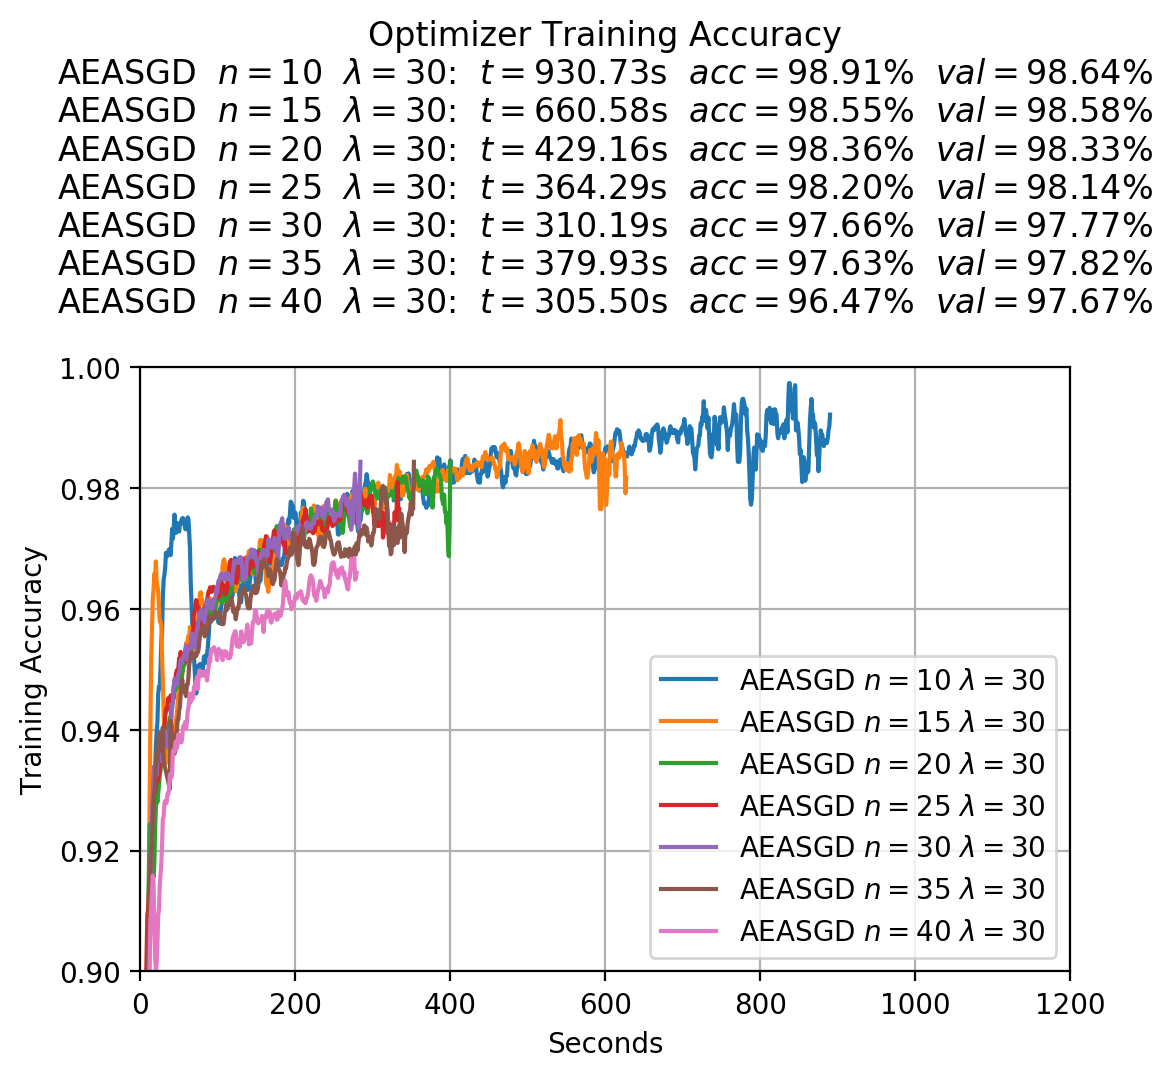
\includegraphics[width=\linewidth]{resources/images/aeasgd_experiments_lambda_30}
    \caption{$\lambda = 30$}
  \end{subfigure}
  \begin{subfigure}{.3\textwidth}
    \centering
    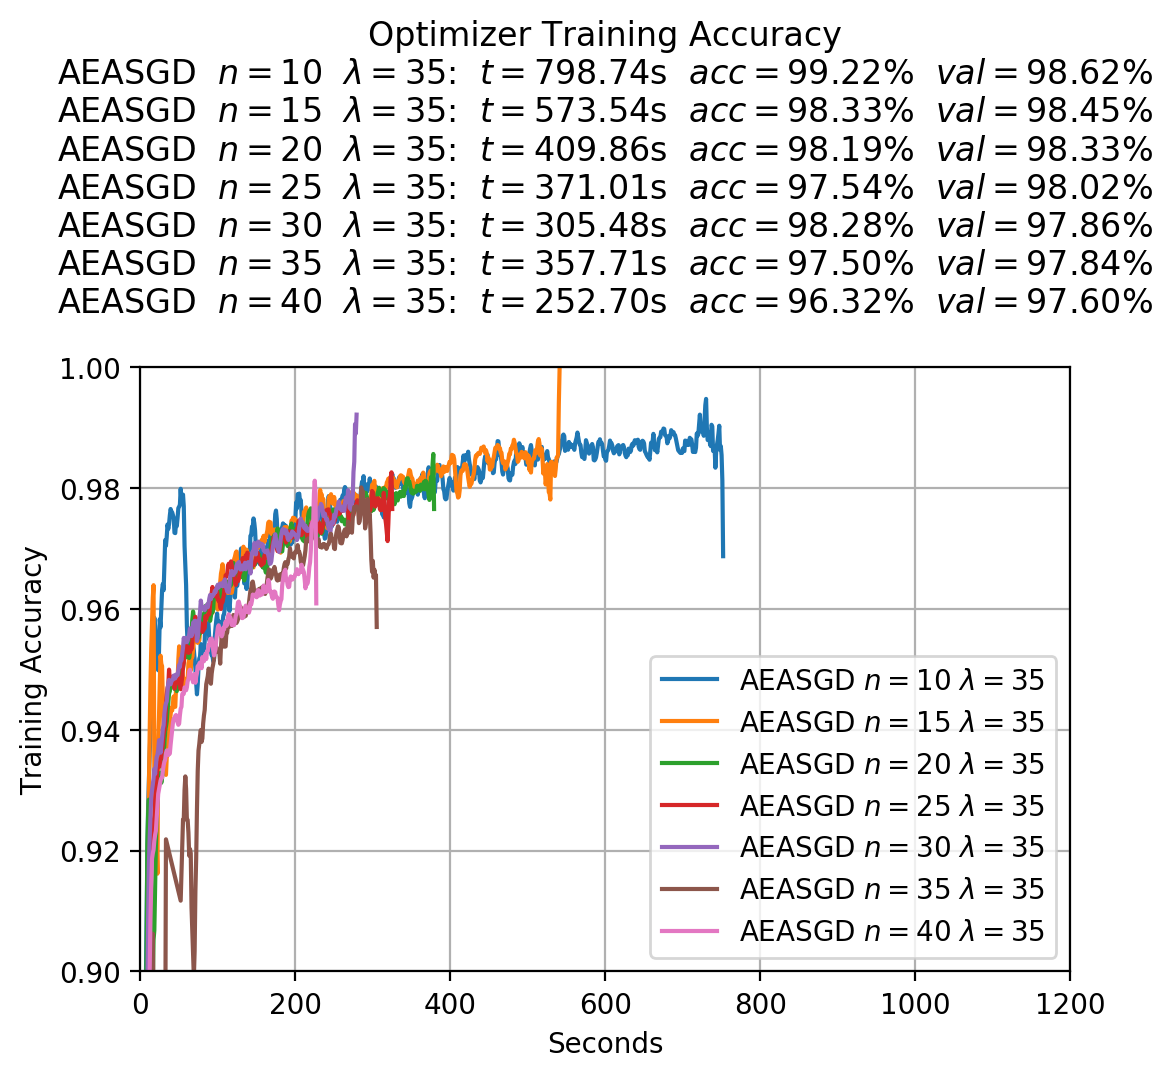
\includegraphics[width=\linewidth]{resources/images/aeasgd_experiments_lambda_35}
    \caption{$\lambda = 35$}
  \end{subfigure}
  \begin{subfigure}{.3\textwidth}
    \centering
    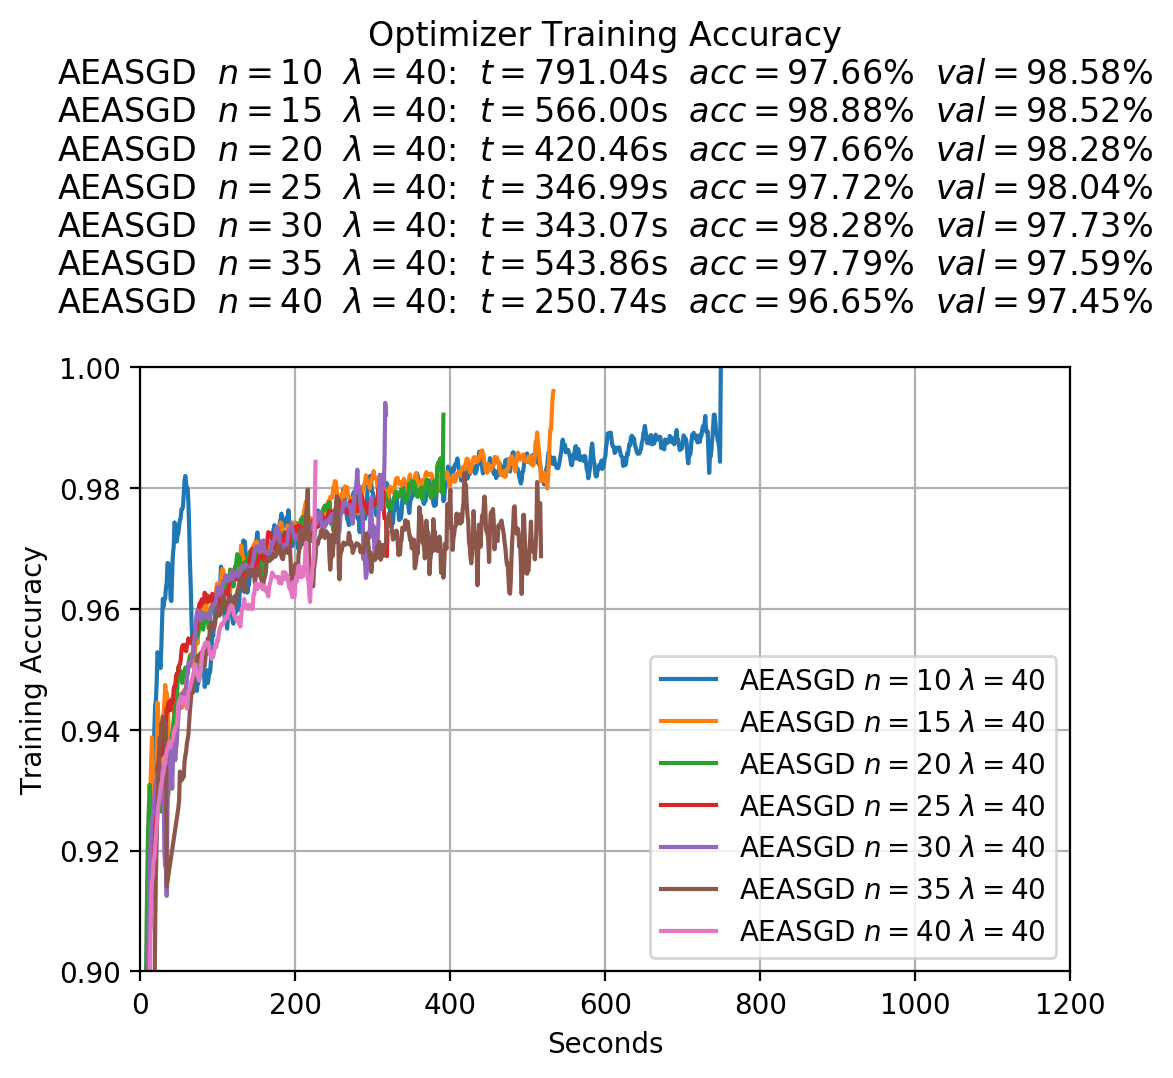
\includegraphics[width=\linewidth]{resources/images/aeasgd_experiments_lambda_40}
    \caption{$\lambda = 40$}
  \end{subfigure}
  \caption{In this experiment we clamp the communication frequency, but vary the number of workers. As in Figure~\ref{fig:aeasgd_experiments_workers}, we do similar observations regarding the flattening of the training accuracy in the precense of a low communication frequency, and a large amount of asynchrony. However, an additional interesting observation which escaped our eye in Figure~\ref{fig:aeasgd_experiments_workers}, is the large ``bump'' in training accuracy for $n = 10$. Nevertheless, this bump is always followed up by a significant reduction in training accuracy. Usually one would expect such behaviour in a configuration with a large amount of asynchrony, but this behaviour is not present is said configurations. Furthermore, the reason why we do not observe significant fluctuations in training accuracy, contrary to \textsc{agn}, is due to hyperparameter $\rho$, which controls the amount of exploration that can be done in terms of \emph{distance}, as discussed in Chapter~\ref{chapter:distributed_deep_learning}.}
  \label{fig:aeasgd_experiments_lambdas}
\end{figure}
